\documentclass[a4paper]{report}

\usepackage[utf8x]{vietnam}
%\usepackage{urwvn}
\usepackage{color}
\usepackage{ifthen}
\usepackage{graphicx}
\usepackage{alltt}
\usepackage{fancybox}
\usepackage{makeidx}
\usepackage{a4}
\usepackage{verbatim}
\usepackage{amsmath}
\usepackage{amsfonts}
%\usepackage{a4-1in}
\usepackage[nodayofweek]{datetime}
\usepackage{longtable}
\usepackage[backref,plainpages=false,pagebackref]{hyperref}
%\usepackage{html}
%\begin{htmlonly}
\usepackage{url}
%\end{htmlonly}
\usepackage{pdfstuff}

\newcommand{\basehtml}{http://theoval.cmp.uea.ac.uk/~nlct/latex}

\makeindex

\newcommand{\scalefac}{1}
\newcommand{\anglerot}{0}

\newcommand{\Index}[1]{#1\index{#1}}
\newcommand{\Indextt}[1]{\texttt{#1}\index{#1@\texttt{#1}}}
\newcommand{\indextt}[1]{\index{#1@\texttt{#1}}}
\newcommand{\cls}[1]{\texttt{#1}\index{class file (\texttt{.cls})!#1@\texttt{#1}}}
\newcommand{\clsopt}[1]{\texttt{#1}\index{Các lựa chọn cho class file!#1@\texttt{#1}}}
\newcommand{\clsfiles}{\index{class file (\texttt{.cls})}}
\newcommand{\tocfile}{\index{file của bảng mục lục (\texttt{.toc})}}
\newcommand{\sty}[1]{\texttt{#1}\index{các gói lệnh (\texttt{.sty})!#1@\texttt{#1}}}
\newcommand{\styfiles}{\index{các gói lệnh (\texttt{.sty})}}
\newcommand{\bst}[1]{\texttt{#1}\index{phong cách tài liệu tham khảo(\texttt{.bst})!#1@\texttt{#1}}}
\newcommand{\bibentry}[1]{\texttt{#1}\index{kiểu danh mục trong tài liệu tham khảo!#1@\texttt{#1}}}
\newcommand{\bibfield}[1]{\texttt{#1}\index{kiểu điền tên cho tài liệu tham khảo!#1@\texttt{#1}}}
\newcommand{\Com}[1]{\texttt{\textbackslash #1}\index{#1@\texttt{\textbackslash #1}}}
\newcommand{\atCom}[1]{\texttt{\textbackslash @#1}\index{"@#1@\texttt{\textbackslash "@#1}}}
\newcommand{\counter}[1]{\texttt{#1}\index{bộ đếm!#1@\texttt{#1}}}
\newcommand{\indexCom}[1]{\index{#1@\texttt{\textbackslash #1}}}
\newcommand{\indexEnv}[1]{\index{  #1@\texttt{#1} ``môi trường''}}
\newcommand{\indexpagestyle}[1]{\texttt{#1}\index{phong cách trang!#1@\texttt{#1}}}
\newcommand{\indexpagenumbering}[1]{\texttt{#1}\index{đánh số trang!#1@\texttt{#1}}}
\newcommand{\leftbrace}{\latexhtml{\Indextt{\symbol{123}}}{\Indextt{\{}}}
\newcommand{\rightbrace}{\latexhtml{\Indextt{\symbol{125}}}{\Indextt{\}}}}
\newcommand{\pgsty}[1]{\texttt{#1}\index{phong cách trang!#1@\texttt{#1}}}
\newcommand{\psatCom}[1]{\texttt{\symbol{92}ps@#1}\index{ps"@#1@\texttt{\symbol{92}ps"@#1}}}

\newcommand{\indexSymbol}[1]{\indextt{\symbol{#1}@{\large\textbackslash\symbol{#1}}}}

%LaTeX2HTML can't handle conditionals
% so make 2 diff commands
\newcommand{\keyword}[1]{{#1}\index{#1}}
\newcommand{\Keyword}[2]{{#1}\index{#2}}

\newcommand{\meta}[1]{\textsf{\slshape #1}}
\newcommand{\envname}[1]{\texttt{#1}\index{#1@\texttt{#1} ``môi trường''}}
\newcommand{\appname}[1]{\texttt{#1}}
\newcommand{\Iappname}[1]{\appname{#1}\index{#1@\texttt{#1}}}
\newcommand{\IAppname}[2]{\appname{#1}\index{#2@\texttt{#2}}}

\newcommand{\BiBTeX}{\textsc{Bib}\TeX\index{BibTeX@\textsc{Bib}\TeX}}
\newcommand{\PDFLaTeX}{PDF\LaTeX\index{PDFLaTeX@PDF\LaTeX}}

\newenvironment{htmlcode}[1][]%
{\par\begin{center}\begin{ttfamily}\begin{minipage}{\textwidth}}%
{\end{minipage}\end{ttfamily}\end{center}}

\newenvironment{htmlbcode}[1][]%
{\par\begin{rawhtml}<table border><td>\end{rawhtml}\begin{center}\begin{ttfamily}\begin{minipage}{\textwidth}}%
{\end{minipage}\end{ttfamily}\par\begin{rawhtml}</td></table>\end{rawhtml}\end{center}}

\newenvironment{htmlresult}[1][]%
{\par\vspace{10pt}\noindent\begin{makeimage}\begin{minipage}{\textwidth}}%
{\end{minipage}\end{makeimage}\par\vspace{10pt}}

\newenvironment{htmldef}[1][]%
{\par\begin{center}\begin{ttfamily}\begin{minipage}{\textwidth}}%
{\end{minipage}\end{ttfamily}\end{center}}

\newcommand{\labelledbox}[2]{\begin{tabular}{r}\doublebox{#1}\\\scriptsize\textsf{#2}\end{tabular}}
\newcommand{\labelled}[2]{\begin{tabular}{r}#1\\\scriptsize\textsf{#2}\end{tabular}}
\newsavebox{\boxcontents}

\newenvironment{ltxcode}[1][0.9\textwidth]%
{\begin{lrbox}{\boxcontents}\begin{minipage}{#1}\begin{ttfamily}}%
{\end{ttfamily}\end{minipage}\end{lrbox}\par\vspace{10pt}\centerline{\labelledbox{\usebox{\boxcontents}}{Input}}\par\noindent\vspace{10pt}}

\newenvironment{ltxbcode}[1][0.9\textwidth]%
{\begin{lrbox}{\boxcontents}\begin{minipage}{#1}\begin{ttfamily}}%
{\end{ttfamily}\end{minipage}\end{lrbox}\par\vspace{10pt}\centerline{\labelledbox{\usebox{\boxcontents}}{Code}}\par\noindent\vspace{10pt}}

\newenvironment{ltxresult}[1][0.9\textwidth]%
{\begin{lrbox}{\boxcontents}\begin{minipage}{#1}}%
{\end{minipage}\end{lrbox}\par\vspace{10pt}\centerline{\labelledbox{\usebox{\boxcontents}}{Output}}\par\noindent\vspace{10pt}}

\newenvironment{ltxdef}[1][0.9\textwidth]%
{\begin{lrbox}{\boxcontents}\begin{minipage}{#1}\begin{ttfamily}}%
{\end{ttfamily}\end{minipage}\end{lrbox}\par\vspace{10pt}\centerline{\labelled{\usebox{\boxcontents}}{Định nghĩa}}\par\vspace{10pt}\noindent}

\newenvironment{definition}[1][0.9\textwidth]%
{\latexhtml{\begin{ltxdef}[#1]}{\begin{htmldef}}}%
{\latexhtml{\end{ltxdef}}{\end{htmldef}}}

%\newenvironment{code}[1][0.9\textwidth]%
%{\latexhtml{\begin{ltxcode}[#1]}{\begin{htmlcode}}}%
%{\latexhtml{\end{ltxcode}}{\end{htmlcode}}}

\newenvironment{code}[1][0.9\textwidth]{\latex{\vspace{10pt}}\begin{htmlcode}}{\end{htmlcode}\vspace{10pt}\noindent}

\newenvironment{bcode}[1][0.9\textwidth]%
{\latexhtml{\begin{ltxbcode}[#1]}{\begin{htmlbcode}}}%
{\latexhtml{\end{ltxbcode}}{\end{htmlbcode}}}

%\newenvironment{result}[1][0.9\textwidth]%
%{\latexhtml{\begin{ltxresult}[#1]}{\begin{htmlresult}}}%
%{\latexhtml{\end{ltxresult}}{\end{htmlresult}}}

\newenvironment{result}[1][0.9\textwidth]{\begin{htmlresult}}{\end{htmlresult}\noindent}

% Need a long table for the required and optional fields (for screen format), but it's
% confusing LaTeX2HTML.

\newenvironment{FieldTabA4}
 {\begin{table}[htbp]
  \caption{Các mục yêu cầu và lựa chọn}\label{tab:reqopt}
  \begin{center}
  \begin{tabular}{lp{0.4\textwidth}p{0.4\textwidth}}
  \bfseries{Loại danh mục} & \bfseries{Các mục yêu cầu} & \bfseries{Các mục lựa chọn}\\
 }
 {
  \end{tabular}
  \end{center}
  \end{table}
 }

\newenvironment{FieldTabScr}
 {\newpage\begin{longtable}{lp{0.4\textwidth}p{0.4\textwidth}}
  \caption{Các mục yêu cầu và lựa chọn}\label{tab:reqopt}\\
  \bfseries{Loại danh mục} & \bfseries{Các mục yêu cầu} & \bfseries{Các mục lựa chọn}\\
  \endfirsthead
  \caption*{Các mục yêu cầu và lựa chọn tiếp theo.}\\
  \bfseries{Loại danh mục} & \bfseries{Các mục yêu cầu} & \bfseries{Các mục lựa chọn}\\
  \endhead
  \endfoot
 }
 {\end{longtable}}

\newenvironment{FieldTab}
 {\ifscreen\begin{FieldTabScr}\else\begin{FieldTabA4}\fi}
 {\ifscreen\end{FieldTabScr}\else\end{FieldTabA4}\fi}

\newenvironment{fieldtab}{\latexhtml{\begin{FieldTab}}{\begin{FieldTabA4}}}{\latexhtml{\end{FieldTab}}{\end{FieldTabA4}}}

\newcommand{\downloadurl}{\basehtml/thesis/examples}

\newcommand{\download}[1]{\htmladdnormallink{download}{\downloadurl/#1.tex}}
\newcommand{\downloadorview}[1]{\htmladdnormallink{download}{\downloadurl/#1.tex} or 
\htmladdnormallink{view}{\downloadurl/#1.html}}

%\begin{latexonly}
\newcommand{\modification}[1]{\underline{\ttfamily #1}}
%\end{latexonly}
\begin{htmlonly}
\newcommand{\modification}[1]{\underline{\em\ttfamily\large #1}}
\end{htmlonly}

\newcommand{\packageurl}{\basehtml/packages}
\newcommand{\packagecls}[1]{\htmladdnormallink{\cls{#1}}{\packageurl/index.html\##1}}
\newcommand{\packagesty}[1]{\htmladdnormallink{\sty{#1}}{\packageurl/index.html\##1}}

\newcommand{\startmenu}[1]{\centerline{{\cmss Start $\rightarrow$ Programs $\rightarrow$ #1}}}
\newcommand{\menu}[1]{{\cmss #1}}

\newenvironment{inlinedef}{\begin{ttfamily}}{\end{ttfamily}}
%\begin{latexonly}
\newcommand{\TeXarchive}{\TeX\ Archive~\cite{texarchive}\index{TeX Archive@\TeX\ Archive}}
%\end{latexonly}
\begin{htmlonly}
\newcommand{\TeXarchive}{\htmladdnormallink{\TeX\ Archive}{http://www.tex.ac.uk/}\index{TeX Archive@\TeX\ Archive}}
\end{htmlonly}

\newcommand{\novices}[1]{\htmladdnormallink{\LaTeX\ for Complete Novices}{\basehtml/novices/#1.html}\latex{~\cite{novices}}}

\renewcommand{\vec}[1]{\boldsymbol{#1}}

\font\cmr=cmr10
\font\cmss=cmss10
\font\cmtt=cmtt10

\newcommand{\pderiv}[2]{\frac{\partial #1}{\partial #2}}
\newcommand{\e}{\mathrm{e}}

\newcommand{\latexbook}{the \LaTeX\ user's guide~\cite{lamport94}}
\newcommand{\Latexbook}{The \LaTeX\ user's guide~\cite{lamport94}}
\newcommand{\latexcomp}{\emph{The \LaTeX\ Companion}~\cite{goossens94}}
\newcommand{\latexguide}{\emph{A Guide to \LaTeX}~\cite{kopka95}}

\pagecolor[gray]{0.8}
\latex{\pagecolor{white}}


\begin{document}

\pagenumbering{alph}% để PDF đếm trang đúng
\stepcounter{page}% PDF  chạy bookmark đúng
\author{\Large\color{red}{Dr Nicola Talbot}\\[4.0ex]Vietnamese Translation by: Thái Phú Khánh Hòa\\[2.5ex] 
\htmladdnormallink{\large\color{blue}{Hóa Học Việt Nam}}{http://www.hoahocvietnam.com}\latex{\ifscreen\\[10pt]\else\\[2in]\includegraphics[height=2in]{ueacrest}\\\fi School of Computing Sciences\\University of East Anglia}}
\title{THIẾT KẾ LUẬN ÁN TỐT NGHIỆP BẰNG \LaTeX{} }
\maketitle

\begin{abstract}
\stepcounter{page}% to get the PDF bookmarks correct
Tài liệu được biên soạn nhằm giúp các nghiên cứu sinh những người muốn sử dụng \LaTeX{} để soạn thảo luận án Tốt Nghiệp của họ.
Nếu bạn chưa  làm quen với \LaTeX{} tôi khuyên bạn trước hết nên đọc \htmladdnormallink{\LaTeX\ for Complete Novices}{\basehtml/novices/novices.html}\latex{~\cite{novices}}.\\[16.0ex]

Các ví dụ được nêu ra trong tài liệu này bạn có thể download từ \htmladdnormallink{thư mục examples }{\basehtml/thesis/examples/index.html} trên website của tác giả. Nếu muốn xem các ví dụ bằng tiếng Việt,  hãy tra cứu ở \htmladdnormallink{VNOSS}{http://www.vnoss.org}\index{VNOSS} chúng tôi sẽ hỏi ý kiến của anh Nguyễn Đại Quí nhằm giúp đỡ việc upload các ví dụ mẫu bằng tiếng Việt, sau khi thiết kế xong luận án của bạn đừng quên gửi file \LaTeX{} nguồn lên \htmladdnormallink{VNOSS}{http://www.vnoss.org} để mọi người tham khảo nhé.
Tài liệu này cũng được tìm thấy ở định dạng khả chuyển (PDF) dưới dạng  \htmladdnormallink{khổ giấy A4 để in ấn}{thesis_a4.pdf} hoặc dưới dạng \htmladdnormallink{slide trình chiếu trên màn hình}{thesis_screen.pdf}.\\[2.0ex]
Bản dịch được nhóm H2VN duyệt  vào: \today.\\[2.0ex]


\begin{latexonly}
\noindent Tài liệu gốc bằng tiếng Anh và các file đính kèm bạn có thể tải về từ:
\url{\basehtml/thesis/thesis.html}. Bản dịch tiếng Việt có thể tải về từ: \htmladdnormallink{H2VN\footnote{Hóa Học Việt Nam}}{http://www.hoahocvietnam.com}\index{H2VN}, \htmladdnormallink{VietTUG\footnote{Nhóm những người Việt Nam sử dụng \TeX{} (Vietnamese TeX Users Group)}}{http://www.viettug.org}\index{VietTUG}, \htmladdnormallink{VNOSS\footnote{Cộng Đồng mã nguồn mở Việt Nam}}{http://www.vnoss.org} hoặc \htmladdnormallink{Vn\TeX\footnote{Dự án Vn\TeX{} tác giả Hàn Thế Thành}.}{http://www.vntex.org}\index{Vn\TeX{}}

\end{latexonly}
\end{abstract}

\latex{\ifscreen\else\pagestyle{headings}\fi}
\pagenumbering{roman}
\setcounter{tocdepth}{2}
\tableofcontents

\clearpage\pagenumbering{arabic}

%%%%%%%%%%%%%%%% INTRODUCTION %%%%%%%%%%%%%%%%%%%%%%%%%%%%

% This is to fix the image file, so the images don't have 
% vrules and hrules.
\def\lthtmlinlinemathB{}
\renewcommand{\lthtmlinlinemathB}[1]{\lthtmlmathtype{#1}\egroup\lthtmlhboxmathA}
\def\lthtmlsetinline{}
\renewcommand{\lthtmlsetinline}{\hbox{\vtop{\vbox{%
  \kern.1em\copy\sizebox}\ifdim\dp\sizebox>0pt\kern.1em\else\kern.3pt\fi
  \ifdim\hsize>\wd\sizebox \fi}}}
\def\lthtmlsetmath{}
\renewcommand{\lthtmlsetmath}{\hbox{\kern-.05em\vtop{\vbox{%
  \kern.1em\kern0.8 pt\hbox{\hglue.17em\copy\sizebox\hglue0.8 pt}}\kern.3pt%
  \ifdim\dp\sizebox>0pt\kern.1em\fi \kern0.8 pt%
  \ifdim\hsize>\wd\sizebox \fi}}}
\def\centerinlinemath{}
\renewcommand{\centerinlinemath}{%
  \dimen1=\ifdim\ht\sizebox<\dp\sizebox \dp\sizebox\else\ht\sizebox\fi
  \advance\dimen1by.5pt 
 \dp\sizebox=\dimen1\ht\sizebox=\dimen1\relax}

\chapter{Giới thiệu}
\label{ch:intro}
\begin{htmlonly}
\index{A@\label{idx:A}\par A\par|phantom}%
\index{B@\label{idx:B}\par B\par|phantom}%
\index{C@\label{idx:C}\par C\par|phantom}%
\index{D@\label{idx:D}\par D\par|phantom}%
\index{E@\label{idx:E}\par E\par|phantom}%
\index{F@\label{idx:F}\par F\par|phantom}%
\index{G@\label{idx:G}\par G\par|phantom}%
\index{H@\label{idx:H}\par H\par|phantom}%
\index{I@\label{idx:I}\par I\par|phantom}%
\index{J@\label{idx:J}\par J\par|phantom}%
\index{K@\label{idx:K}\par K\par|phantom}%
\index{L@\label{idx:L}\par L\par|phantom}%
\index{M@\label{idx:M}\par M\par|phantom}%
\index{N@\label{idx:N}\par N\par|phantom}%
\index{O@\label{idx:O}\par O\par|phantom}%
\index{P@\label{idx:P}\par P\par|phantom}%
\index{Q@\label{idx:Q}\par Q\par|phantom}%
\index{R@\label{idx:R}\par R\par|phantom}%
\index{S@\label{idx:S}\par S\par|phantom}%
\index{T@\label{idx:T}\par T\par|phantom}%
\index{U@\label{idx:U}\par U\par|phantom}%
\index{V@\label{idx:V}\par V\par|phantom}%
\index{W@\label{idx:W}\par W\par|phantom}%
\index{X@\label{idx:X}\par X\par|phantom}%
\index{Y@\label{idx:Y}\par Y\par|phantom}%
\index{Z@\label{idx:Z}\par Z\par|phantom}%
\index{ @\htmlref{A}{idx:A} "| \htmlref{B}{idx:B} "| \htmlref{C}{idx:C} "| \htmlref{D}{idx:D} "| \htmlref{E}{idx:E} "| \htmlref{F}{idx:F} "| \htmlref{G}{idx:G} "| \htmlref{H}{idx:H} "| \htmlref{I}{idx:I} "| \htmlref{J}{idx:J} "| \htmlref{K}{idx:K} "| \htmlref{L}{idx:L} "| \htmlref{M}{idx:M} "| \htmlref{N}{idx:N} "| \htmlref{O}{idx:O} "| \htmlref{P}{idx:P} "| \htmlref{Q}{idx:Q} "| \htmlref{R}{idx:R} "| \htmlref{S}{idx:S} "| \htmlref{T}{idx:T} "| \htmlref{U}{idx:U} "| \htmlref{V}{idx:V} "| \htmlref{W}{idx:W} "| \htmlref{X}{idx:X} "| \htmlref{Y}{idx:Y} "| \htmlref{Z}{idx:Z}\par|phantom}%
\end{htmlonly}

Trong các trường Đại Học ở nước ta hiện nay qui định về cách trình bày luận án tốt nghiệp có thể khác với phong cách của các trường trên thế giới. Nhìn chung luận án của các sinh viên trong nước trông rất thiếu chuyên nghiệp và còn mang nặng tính hình thức nhiều, ví dụ như khi bạn làm luận án bạn phải để tên giáo viên hướng dẫn ở phía trên của người thực hiện thay vì chỉ đề cập đến tên của họ vào phần ``Cảm Ơn''. Thậm chí phong cách trình bày luận án là do mỗi trường tự đề ra mà không có một định dạng chuẩn nào trong cả nước, có đôi khi một vài người phản biện họ cãi nhau về cách trình bày tài liệu của sinh viên. Hầu hết người ta khi làm luận án thường  sử dụng \emph{MS Word} hay viết tay rồi thuê các dịch vụ văn phòng đánh máy lại, và công việc chỉnh sửa rất mất nhiều thời gian. Gần đây một số sinh viên ở các trường Đại Học Quốc Gia đã quan tâm đến \LaTeX{} và sử dụng nó để soạn thảo tài liệu khoa học, đây là một dấu hiệu rất đáng mừng.

Hiện nay các nghiên cứu sinh khoa học cũng như sinh viên các trường đại học thường được khuyến cáo sử dụng \LaTeX{} để soạn thảo luận án tốt nghiệp, đặc biệt là khi luận án của họ có liên quan đến nhiều biểu thức toán học. Tài liệu được biên soạn với mục đích là một bài giới thiệu ngắn về cách thiết kế và định dạng tài liệu của bạn và cách  định nghĩa các kiểu trang, đầu đề của chương, khác với phong cách trình bày cổ điển \ldots Nếu bạn bạn chưa bao giờ đụng đến \LaTeX{} thì bạn nên tìm đọc \novices{novices} và một số tài liệu Việt Ngữ liên quan có thể tìm thấy ở \htmladdnormallink{VietTUG}{http://www.viettug.org} hoặc tham vấn các chuyên gia về \TeX{} trên \htmladdnormallink{VNOSS}{http://www.vnoss.org}. Tài liệu này viết cho những người đã có những kiến thức cơ bản về \LaTeX{}.\\

%%\begin{latexonly}
%Throughout this document, source code is illustrated by a typewriter font in a box labelled ``Input'' or ``Code'' and
%the corresponding output is placed in a box labelled ``Output''.  For example:\\[10pt]
%Sample Code:
%%\end{latexonly}
%\begin{htmlonly}
\noindent Xuyên suốt tài liệu này, mã nguồn sẽ được minh họa dưới dạng như sau:

%\end{htmlonly}
\begin{code}
\begin{verbatim}
Đây là một \textbf{ví dụ}.
\end{verbatim}
\end{code}%
\noindent
%\latexhtml{Resulting output:}{The corresponding output is illustrated as follows:}
Và kết quả tương ứng sẽ được minh họa dưới dạng sau:

\begin{result}
Đây là một \textbf{ví dụ}.
\end{result}%
Các định nghĩa về lệnh sẽ được dùng font chữ đánh máy dưới dạng như sau:

\begin{definition}
\verb|\documentclass[|\meta{tùy chọn}\verb|]{|\meta{file viết riêng cho từng lớp tài liệu}\verb|}|
\end{definition}

%%%%%%%%%%%%%%%%%%%%% Getting Started %%%%%%%%%%%%%%%%%%%%%%%%%%%%

\chapter{Bắt đầu như thế nào}

Nếu bạn được ai đó chỉ bảo dùng một class (lớp tài liệu) file nào đó, thì hãy cứ làm theo như những gì mà người có kinh nghiệm hướng dẫn bạn, còn nếu không tôi khuyên bạn nên dùng file của lớp \cls{report}. Trước khi bạn tiến hành soạn thảo tài liệu nên chú ý rằng kiểu cấu trúc tài liệu nào bạn nên chọn. Trừ khi giáo viên hướng dẫn của bạn yêu cầu, nếu không tôi khuyên bạn trước hết nên lập ra sườn của tài liệu mà ít nhiều trông giống như dưới đây:
  
\label{ex:thesis1}
\verbatiminput{examples/thesis1.tex}
\html{(Bạn có thể \download{thesis1} một bản copy của file này nếu muốn.)}
Nếu bạn đã download file nguồn của ví dụ này, nó sẽ giúp bạn xác định rằng tài liệu của bạn được định dạng đúng trước khi bạn bắt đầu nhập nội dung của tài liệu.


%%%%%%%%%%%%%%%%% Splitting Document %%%%%%%%%%%%%%%%%%%%%%%%%%%%%

\chapter{Chia nhỏ một tài liệu lớn ra nhiều file }

Một số người thích đặt mỗi chương trong một tài liệu lớn thành một file riêng biệt. Bạn có thể làm việc này bằng cách sử dụng dòng lệnh sau:

\begin{definition}
\Com{include}\{\meta{tên của file}\}
\end{definition}%
Nếu bạn chỉ muốn làm việc với một hay hai chương, bạn có thể báo cho \LaTeX{} biết để đính kèm những file này với lệnh:

\begin{definition}
\Com{includeonly}\{\meta{liệt kê tên file}\}
\end{definition}%
ở phần khai báo nơi mà \meta{tên của các file} mà bạn muốn đính vào cách nhau bằng dấu phẩy.
\LaTeX{} sẽ đọc tất cả các thông tin về tham chiếu chéo đối với những chương  đã không được đính vào danh sách, nhưng sẽ không cập nhật chúng vào file DVI. Có một lợi điểm với việc này là nếu có một số lượng lớn hình ảnh trong chương kết quả của bạn, mà bạn không muốn đính kèm theo khi làm việc, vì thời gian biên dịch sẽ lâu hơn, đây là một mẹo nhỏ. Tuy nhiên bạn vẫn có thể tham chiếu đến các hình ảnh trong những chương bạn không đính kèm theo khi mà bạn biên dịch tài liệu với \LaTeX{} sau khi bỏ lệnh \Com{includeonly}.\\[2.0ex]

Ví dụ \hyperref{ở chương trước}{được nêu ra trong Chương~}{}{ex:thesis1}{} bây giờ có thể chia nhỏ ra làm nhiều file:\\

\noindent \textbf{File} \htmladdnormallink{thesis.tex}{examples/thesis2.tex}:

\verbatiminput{examples/thesis2.tex}

\noindent \textbf{File} \htmladdnormallink{gioithieu.tex}{examples/gioithieu.tex}:

\verbatiminput{examples/gioithieu.tex}

\noindent \textbf{File} \htmladdnormallink{vaode.tex}{examples/vaode.tex}:

\verbatiminput{examples/vaode.tex}

\noindent \textbf{File} \htmladdnormallink{phuongphap.tex}{examples/phuongphap.tex}:

\verbatiminput{examples/phuongphap.tex}

\noindent \textbf{File} \htmladdnormallink{ketqua.tex}{examples/ketqua.tex}:

\verbatiminput{examples/ketqua.tex}

\noindent \textbf{File} \htmladdnormallink{ketluan.tex}{examples/ketluan.tex}:

\verbatiminput{examples/ketluan.tex}

Nếu bạn chỉ muốn làm việc với chương Phương Pháp và chương Kết Quả bạn chỉ cần đặt những lệnh sau vào phần khai báo.

\begin{verbatim}
\includeonly{phuongphap,ketqua}
\end{verbatim}

%%%%%%%%%%%%%%%%% Changing the Document Style %%%%%%%%%%%%%%%%%%%%%%%%%%

\chapter{Thay đổi phong cách tài liệu}
\label{ch:mythesis}

Bạn có thể định nghĩa lại \Com{Chương}, \Com{mục} để thay đổi đầu đề của trang trong tài liệu. Nếu bạn muốn thay đổi thì tôi khuyên rằng bạn tạo một file riêng cho lớp tài (class file) liệu mới. Để làm việc này có hai lý do chính:
trước hết, một số lệnh có liên quan sử dụng một  ký tự \verb|@| mà nó sẽ thay đổi tính năng của nó tùy thuộc vào việc nó có được dùng trong một lớp hay gói lệnh hay trong một file văn bản thông thường, và thứ hai là nếu bạn đặt tất cả các lệnh trong tài liệu gốc của bạn, điều này sẽ quấy rối bộ máy kiểm tra chính tả hay bộ đếm từ\footnote{Để biết thêm thông tin về bộ đếm từ văn bản hãy đọc tài liệu hướng dẫn của class file \packagecls{cmpreprt}}.

Như vậy bạn có nên tạo ra một gói lệnh hay một class file hay không? Các gói lệnh nên được thiết kế độc lập với class file. Chẳng hạn như, gói lệnh \sty{graphicx} làm việc không phụ thuộc vào việc bạn có đang dùng \cls{report}, \cls{article}, \cls{slide} class file hay không. Nếu lệnh hay môi trường mà bạn muốn định nghĩa theo phong cách riêng của mình, khác so với các class file sẵn có thì bạn nên tạo một class file mới dựa trên phong cách tài liệu mà bạn muốn hướng đến. Còn nếu bạn muốn định nghĩa kiểu trình bày chương mục mới và phong cách mới, mà nó sẽ độc lập với tất cả các phần còn lại của tài liệu, thì có nghĩa là nó phụ thuộc vào class file. Do vậy bạn nên tạo một  class file mới bằng việc chỉnh sửa file đã có, sẽ tiết kiếm được nhiều công sức hơn là tạo ra một gói lệnh mới.

Hãy xem ví dụ dưới đây. Nếu bạn muốn tạo một lớp mới gọi là \cls{mythesis} bạn cần tạo một file gọi là \texttt{mythesis.cls}, và phần mở đầu trong file của bạn sẽ trông giống như thế này:

\begin{verbatim}
\NeedsTeXFormat{LaTeX2e}
\ProvidesClass{mythesis}
\end{verbatim}
Kế đến bạn phải xác định được bạn sẽ làm gì với các lựa chọn trong file \cls{report}. Khi mà chúng ta không cần định nghĩa lại bất cứ lựa chọn nào có sẵn trong file đã được định nghĩa trước đó thì đơn giản hãy bỏ qua các lựa chọn trong \cls{report} class file:

\begin{verbatim}
\DeclareOption*{\PassOptionsToClass{\CurrentOption}{report}}
\end{verbatim}
Sau khi tất cả các lựa chọn đã được khai báo chúng cần được xử lý:
\begin{verbatim}
\ProcessOptions
\end{verbatim}
Bây giờ lớp \cls{report} cần được nạp lại:
\begin{verbatim}
\LoadClass{report}
\end{verbatim}
dòng cuối cùng trong file của bạn cần có lệnh:
\begin{verbatim}
\endinput
\end{verbatim}
Nội dung của class file mới này sẽ được chèn vào giữa các lệnh \Com{LoadClass}\verb|{report}| và \Com{endinput}. Sau đó bạn cần chỉnh sửa lại mã nguồn  của bạn, file \texttt{thesis.tex} sẽ dùng class file mới được tạo này.

\begin{verbatim}
\documentclass[a4paper]{mythesis}
\end{verbatim}

\section{Cải biến đối tượng văn bản}

Tập tin \cls{report}  định nghĩa nhiều lệnh mà chúng dùng để in ra các \emph{từ} như:``Mục Lục'',``Chương'',``Tài liệu tham khảo''. Các lệnh này và những giá trị mặc định của chúng được liệt kê trong  Bảng~\ref{tab:names}.

\begin{table}[hbt]
\caption{Tên mặc định được in ra với các lệnh tương ứng}
\label{tab:names}
\begin{center}
\begin{tabular}{ll}
\Com{contentsname} & Mục lục\\
\Com{listfigurename} & Danh sách hình ảnh\\
\Com{listtablename} & Danh sách các bảng \\
\Com{bibname} & Tài liệu tham khảo\\
\Com{indexname} & Chỉ mục\\
\Com{figurename} & Hình\\
\Com{tablename} & Bảng\\
\Com{partname} & Phần\\
\Com{chaptername} & Chương\\
\Com{appendixname} & Phụ lục\\
\Com{abstractname} & Tóm tắt nội dung
\end{tabular}
\end{center}
\end{table}

Giả sử rằng bạn muốn các hình ảnh và bảng biểu được gán nhãn là H.\ và B.\ thay cho Hình và Bảng thì bạn có thể thêm các dòng sau vào \texttt{mythesis.cls}:

\begin{verbatim}
\renewcommand{\figurename}{H.}
\renewcommand{\tablename}{B.}
\end{verbatim}

%%%%%%%%%%%%%%%%% redefining \section etc %%%%%%%%%%%%%%%%%%%

\section{Thay đổi đầu đề trang của các mục}

Bạn có thể tùy biến phong cách trình bày cho tiêu đề trang trong từng chương mục bằng cách định nghĩa lại các lệnh tương ứng 
\Com{section},
\Com{subsection} \ldots  dùng lệnh:
\begin{definition}
\atCom{startsection}\{\meta{type}\}\{\meta{level}\}\{\meta{indent}\}\{\meta{beforeskip}\}\{\meta{afterskip}\}\{\meta{style}\}
\end{definition}%
\noindent Sáu argument  có nghĩa như sau:
\begin{description}
\item[\normalfont\meta{type}]
Kiểu sắp xếp các mục trong tài liệu.  Một trong số đó là: \texttt{Mục chính},
\texttt{mục phụ thứ nhất}, \texttt{mục phụ thứ 2}, \texttt{đoạn văn chính} hoặc \texttt{đoạn văn phụ}.
(Chú ý không có gạch xiên \backslash)

\item[\normalfont\meta{level}]
Đây là thứ tự các mục, đã được mô tả trong Bảng~\ref{tab:secnum}.

\item[\normalfont\meta{indent}]
Đây là độ dài một khoảng trắng mà chữ đầu tiên của hàng cách lề trái của trang.

\item[\normalfont\meta{beforeskip}]
Là giá trị tuyệt đối của \meta{beforeskip}  xác định khoảng cách theo chiều dọc được chừa ra trước tiêu đề trang. Nếu \meta{beforeskip} là âm thì đoạn văn đầu tiên theo sau tiêu đề trang sẽ không dời vào một chữ ở hàng đầu tiên.

\item[\normalfont\meta{afterskip}]
 Giá trị tuyệt đối của \meta{afterskip}  xác định khoảng cách theo chiều dọc chừa ra sau phần tiêu đề trang. Nếu \meta{afterskip}  có giá trị âm thì văn bản theo sau lệnh đặt tiêu đề xuất hiện thẳng hàng với phần tiêu đề trang.

\item[\normalfont\meta{style}]
Argument \meta{style}  là các khai báo được yêu cầu để thiết  lập phong cách của tiêu đề trang. (ví dụ
\Com{itshape} tiêu đề trang sẽ được in chữ nghiêng.) 

\end{description}

\begin{table}[hbt]
\caption{Thứ tự các mục}
\label{tab:secnum}
\begin{center}
\begin{tabular}{lr}
phần & -1\\
chương & 0\\
mục & 1\\
mục con thứ nhất & 2\\
mục con thứ 2 & 3\\
đoạn văn & 4\\
đoạn văn con & 5
\end{tabular}
\end{center}
\end{table}

\noindent Giả sử bạn muốn thay đổi tiêu đề trang để in ra font chữ nghiêng bạn có thể làm như sau:
\begin{verbatim}
\renewcommand{\section}{\@startsection
{section}%                           % tên
{1}%                                     % thứ tự
{0mm}%                               % thụt đầu dòng
{-\baselineskip}%                 % trước khi cách
{0.5\baselineskip}%             % sau khi cách
{\normalfont\large\itshape}} % kiểu font
\end{verbatim}
\noindent Tham khảo \latexguide{} để có thêm thông tin.\\[2.0ex]

\niondent Có một bộ đếm gọi là \Indextt{secnumdepth} điều khiển thứ tự của các mục được đánh số. Thứ tự sẽ tương ứng với những gì nêu trong Bảng~\ref{tab:secnum}. Theo mặc định thì giá trị này là 2, nên chỉ có các phần, chương, mục và mục con thứ nhất có các số liên đới.
Bạn có thể dùng \Com{setcounter} để thay đổi giá trị của \Indextt{secnumdepth}.  
Ví dụ như nếu bạn muốn lệnh \Com{paragraph} in ra một số làm như sau:
\begin{verbatim}
\settocounter{secnumdepth}{4}
\end{verbatim}

%%%%%%%%%%%%%%%% redefining \chapter and \part %%%%%%%%%%%%

\section{Thay đổi tiêu đề chương}

Nếu bạn muốn thay đổi phong cách của tiêu đề cho các phần hay các chương bạn không thể dùng lệnh \atCom{startsection}. Thay vào đó bạn dùng lệnh \Com{secdef}. Nếu bạn nạp file \texttt{report.cls} vào trong editor của bạn, bạn sẽ thấy rằng cả hai lệnh \Com{part} và \Com{chapter} dùng \Com{secdef}. Định nghĩa về \Com{chapter} có dòng sau:

\begin{verbatim}
\secdef\@chapter\@schapter
\end{verbatim}
và \Com{part} có dòng sau:
\begin{verbatim}
\secdef\@part\@spart
\end{verbatim}
Argument đầu tiên trong \Com{secdef} thông báo cho \LaTeX{} cần thực hiện những gì nếu phiên bản chưa được đánh dấu sao được dùng, và argument thứ hai thông báo cho \LaTeX{} cần làm gì nếu như phiên bản đã đánh dấu sao được sử dụng. Do vậy lệnh

\begin{verbatim}
\chapter{Giới thiệu}
\end{verbatim}
sẽ dùng lệnh \atCom{chapter}, trái lại lệnh

\begin{verbatim}
\chapter*{Lời cảm ơn}
\end{verbatim}
sẽ dùng lệnh \atCom{schapter}.
Lệnh \atCom{chapter} và \atCom{schapter} dùng  lần lượt các lệnh \atCom{makechapterhead} và \atCom{makeschapterhead}, để định dạng tiêu đề chương, và nếu bạn muốn thay đổi định dạng chương, bạn cần định nghĩa lại  các lệnh \atCom{makechapterhead}
và \atCom{makeschapterhead}.  Cách dễ nhất để làm điều này là tìm mã  của những lệnh này trong \texttt{report.cls}  và copy chúng vào  trong class file của bạn, \texttt{mythesis}, \htmlref{đã đề cập ở trên}{ch:mythesis},  và chỉnh sửa các lệnh định dạng thích hợp.

Ví dụ, giả sử rằng bạn muốn có một hàng xuất hiện trên và dưới tiêu đề chương và tiêu đề sẽ xuất hiện ở dạng chữ in hoa nhỏ (thông thường trên tiêu đề trang, tên của mục xuất hiện ở trang bên trái và tên chương xuất hiện ở trang bên phải) bạn làm như sau:

\begin{verbatim}
\renewcommand{\@makechapterhead}[1]{%
  \vspace*{50\p@}%
  {\parindent \z@ \raggedright \normalfont
    \hrule                                        % đường kẻ ngang
    \vspace{5pt}%                 % thêm khoảng cách theo chiều dọc
    \ifnum \c@secnumdepth >\m@ne
      \huge\scshape \@chapapp\space \thechapter % đánh số chương
        \par\nobreak
        \vskip 20\p@
    \fi
    \interlinepenalty\@M
    \Huge \scshape #1\par                         % tiêu đề chương
    \vspace{5pt}%                                 % thêm khoảng cách chiều dọc
    \hrule                                        % đường kẻ ngang
    \nobreak
    \vskip 40\p@
  }}

\renewcommand{\@makeschapterhead}[1]{%
  \vspace*{50\p@}%
  {\parindent \z@ \raggedright
    \normalfont
    \hrule                                        % đường kẻ ngang 
    \vspace{5pt}%                                 % thêm khoảng cách chiều dọc
    \interlinepenalty\@M
    \Huge \scshape #1\par                         % tiêu đề chương
    \vspace{5pt}%                                 % thêm khoảng cách chiều dọc
    \hrule                                        % đường kẻ ngang 
    \nobreak
    \vskip 40\p@
  }}
\end{verbatim}

Bạn có thể download file \htmladdnormallink{mythesis.cls}{examples/mythesis.cls} có đính kèm tất cả các ví dụ trong chương này.

%%%%%%%%%%% \addcontentsline %%%%%%%%%%%

\section{Thêm vào phần mục lục}

Các phiên bản của các lệnh đánh số các mục không được thêm phần mục lục điều này đã được mặc định trước, nhưng bạn vẫn có thể thêm vào, sử dụng:

\begin{definition}
\Com{addcontentsline}\{\meta{file}\}\{\meta{type}\}\{\meta{văn bản}\}
\end{definition}%
\begin{description}
\item[\normalfont\meta{file}]
Đây là phần mở rộng của file trong đó nội dung được ghi lên.
Do vậy đây sẽ là \Indextt{toc} (table of contents) cho phần mục lục còn \Indextt{lof} (list of figures) là danh sách hình ảnh và \Indextt{lot} (list of tables) là danh sách các bảng.

\item[\normalfont\meta{type}]
Đây là loại đối tượng bạn đưa vào phần nội dung như chương, mục, hình ảnh.

\item[\normalfont\meta{text}]
Đây là phần văn bản trong nội dung tài liệu
\end{description}

\noindent Chẳng hạn như, mục tài liệu tham khảo được tạo ra bằng việc dùng các phiên bản đã đánh dấu sao của lệnh \Com{chapter} nên nó không cần thêm vào phần mục lục nữa, bạn có thể tiến hành.

\begin{verbatim}
\addcontentsline{toc}{chapter}{\bibname}
\end{verbatim}

\noindent Bộ đếm \Indextt{tocdepth} điều khiển mức độ thụt vào của các mục trong bảng mục lục. Thứ tự  tương ứng của các mục được liệt kê ở Bảng~\ref{tab:secnum}.

\noindent Class file \cls{report} thiết lập cho \Indextt{tocdepth}  nằm ở thứ tự số 2, có nghĩa là chỉ có các phần, các chương, mục và mục nhỏ sẽ được thêm vào bảng mục lục. Bạn có thể dùng  lệnh \Com{setcounter} để thay đổi giá trị của \Indextt{tocdepth}. Chẳng hạn như để gắn cả mục con thứ 2, đoạn văn và đoạn văn con vào bảng mục lục làm như sau:


\begin{verbatim}
\setocounter{tocdepth}{5}
\end{verbatim}


%%%%%%%%%%%%% Tái định nghĩa phong cách trang %%%%%%%%%%%%%%%%%%%%%%%

\section{Định nghĩa một phong cách dàn trang mới}
\label{sec:newps}

Có hai phong cách dàn trang được \LaTeX\footnote{ hầu hết các lass file chuẩn bao gồm \cls{report} và định nghĩa phong cách trang \pgsty{headings} và \pgsty{myheadings}} định nghĩa sẵn đó là \pgsty{empty} và \pgsty{plain}. Các cách dàn trang này có thể được lựa chọn bằng cách dùng một trong hai lệnh sau:

\begin{definition}
\Com{pagestyle}\{\meta{style}\}
\end{definition}
để thay đổi phong cách trang  ``từ điểm này cho đến hết tài liệu'', hoặc
\begin{definition}
\Com{thispagestyle}\{\meta{style}\}
\end{definition}
để thay đổi cho một trang xác định nào đó.\\[1.0ex]

\noindent Cả hai lệnh này đều gọi lệnh \verb|\ps@|\meta{style} để thực hiện công việc, và cũng chính lệnh này định nghĩa lại cách hiển thị của header và footer\footnote{\emph{khỏi phải bàn chắc ai cũng biết header và footer là gì rồi}}. Do đó \verb|\pagestyle{plain}| gọi lệnh \psatCom{plain}  đến lượt gọi các lệnh định nghĩa lại header và footer, và \verb|\pagestyle{empty}| gọi lệnh \psatCom{empty} \ldots
  
\noindent Để định nghĩa một phong cách trang mới mà ở đây chúng ta gọi là \pgsty{thesis}, trước hết bạn cần định nghĩa một lệnh được gọi là \psatCom{thesis}. Kể từ khi tên lệnh chứa một ký tự \verb|@|, định nghĩa cần nhập vào file phong cách hay file lớp tài liệu.
  
\noindent Header và footer cho trang lẻ và trang chẵn có thể được xác định bằng việc định nghĩa lại các lệnh sau:\\

\atCom{oddhead}, \atCom{evenhead}, \atCom{oddfoot} và \atCom{evenfoot}.\\

\noindent Giả sử rằng bạn muốn trang mới có header rỗng và footer có chứa số trang với hai dấu gạch ngang hai bên (ví dụ \latexhtml{\ifscreen\linebreak\fi-\thepage-}{-10-} ) ở chính giữa chân trang bạn có thể làm như sau:

\begin{verbatim}
\newcommand{\ps@thesis}{
   \renewcommand{\@oddhead}{}%     header trống
   \renewcommand{\@evenhead}{}%    header trống
   \renewcommand{\@oddfoot}{\hfill-\thepage-\hfill}%     
   \renewcommand{\@evenfoot}{\hfill-\thepage-\hfill}%     
}
\end{verbatim}

\noindent Chú ý rằng khi bạn dùng mặc định lựa chọn \clsopt{oneside} cho class file \cls{report} thì chỉ  có các lệnh \atCom{oddhead} và \atCom{oddfoot} sẽ được kích hoạt. Còn nếu bạn muốn đánh số trang chẵn và lẻ khác nhau thì bạn phải nhớ là dùng lựa chọn \clsopt{twoside}\footnote{nhưng lựa chọn kỳ cục này không thích hợp trong một luận án}.

\noindent Bạn cũng có thể tùy biến phong cách trang bằng cách sử dụng gói lệnh \sty{fancyhdr} của Piet~van~Oostrum. Tham khảo thêm ở \latexguide{}.
\noindent Trừ khi bạn được yêu cầu, còn không tôi khuyên bạn dùng  phong cách \pgsty{headings}.



%%%%%%%%%%%%%%%  dùng BiBTeX %%%%%%%%%%%%%%%%%%%%%%%

\chapter{Tạo danh mục cho tài liệu tham khảo}

Khi bạn soạn một tài liệu lớn giống như là luận án Tiến Sĩ chẳng hạn, tôi thật sự muốn khuyên bạn rằng bạn dùng \BiBTeX{} tốt hơn là đánh danh sách tài liệu tham khảo trong môi trường \envname{thebibliography}. Nếu bạn dùng \BiBTeX{}:

\begin{enumerate}
\item Chỉ những tham khảo mà bạn trích dẫn được phép cho vào trong danh sách thao khảo.
(Những người phản biện hay bắt lỗi những tài liệu tham khảo không được liệt kê.)

\item Các tài liệu tham khảo được hiển thị theo phong cách nhất quán.

\item Danh mục có thể được đặt theo thứ tự trích dẫn hay theo thứ tự của bảng chữ cái.

\item Phong cách trình bày có thể dễ dàng thay đổi bằng cách dùng các file phong cách (sty file) khác nhau cho mục tài liệu tham khảo.

\end{enumerate}

Có thể bạn đã xem qua \htmladdnormallink{ví dụ}{examples/thesis1.tex} ở Chương~\ref{ex:thesis1} có các dòng sau:

\begin{verbatim}
\bibliographystyle{plain}
\bibliography{thesis}
\end{verbatim}
Và lệnh
\begin{definition}
\Com{bibliographystyle}\{\meta{style}\}
\end{definition}%
xác định rằng trong đó trong đó file phong cách nào của \BiBTeX{}         (\texttt{.bst}) để dùng không mà không mở rộng. Ví dụ ở trên dùng \texttt{plain.bst} và lệnh

\begin{definition}
\Com{bibliography}\{\meta{database}\}
\end{definition}%
để xác định cơ sở dữ liệu nào được sử dụng. Ví dụ trên dùng cơ sở dữ liệu trong file \texttt{thesis.bib}, đây là file mà chúng ta cần tạo.
Từ khi tài liệu hiện tại không có bất kỳ một lệnh trích dẫn nào \Com{cite}, và file \texttt{thesis.bib}  chưa được tạo, do đó file DVI sẽ không có danh mục tham khảo.
Có nhiều kiểu trình bày danh mục tài liệu tham khảo nhưng những cách cơ bản đó là:


\begin{description}
\item[\bst{abbrv}] Danh mục được lưu theo thứ tự alphabe và tên của tác giả được viết tắt, kế đó là ngày tháng và tên tạp chí. Bạn có thể so sánh qua những hình ảnh ở những trang sau.

\item[\bst{alpha}] Danh mục được lưu trữ theo thứ tự alphabe với trích dẫn là tên và họ của tác giả, và năm xuất bản thay vì là số.

\item[\bst{plain}] Danh mục được lưu theo thứ tự alphabe và trích dẫn theo số.

\item[\bst{unsrt}]  Danh mục được lưu theo sự trích dẫn mà sự trích dẫn thể hiện bằng một số.
\end{description}
Xem thêm trong \latexguide\ hoặc \latexcomp\ để biết thêm chi tiết về những phong cách trình bày khác về Tài liệu tham khảo, hãy thảo luận với giáo viên hướng dẫn của bạn về một phong cách trình bày cụ thể nào đó mà bạn nên dùng.


Danh mục trong cơ sở dữ liệu của tài liệu tham khảo nên có dạng như sau:

\vbox{\begin{alltt}
@\meta{Thể loại danh mục}\{\meta{từ khóa},
   \meta{vùng điền tên} = "\meta{văn bản}",
       \html{.}
       \latexhtml{\vdots}{.}
       \html{.}
   \meta{vùng điền tên} = "\meta{văn bản}"
\}
\end{alltt}}
\noindent trong đó \meta{loại danh mục} xác định thể loại của danh mục (ví dụ book hoặc article).
Các kiểu danh mục chuẩn được liệt kê trang Bảng~\ref{tab:entrytype}. 


\begin{table}[htbp]
\caption{Các kiểu danh mục BibTeX chuẩn}
\label{tab:entrytype}
\begin{center}
\begin{tabular}{ll}
\bibentry{article} & Bài báo từ các tạp chí\\
\bibentry{book} & Sách đã xuất bản\\
\bibentry{booklet} & Các đề tài được in không có xuất bản\\
\bibentry{conference} & Tương tự như \texttt{inproceedings }\\
\bibentry{inbook} & Phần, chương, mục trong một quyển sách\\
\bibentry{incollection} & Một chương trong một quyển sách có tác giả và tiêu đề riêng\\
\bibentry{inproceedings} & Một bài báo cáo được lưu trong biên bản của một hội nghị\\
\bibentry{manual} & Tài liệu kỹ thuật\\
\bibentry{mastersthesis} & Luận án Thạc Sĩ\\
\bibentry{misc} & Công việc không theo qui định chuẩn\\
\bibentry{phdthesis} & Luận án Tiến Sĩ\\
\bibentry{proceedings} & Biên bản hội nghị\\
\bibentry{techreport} & Báo cáo được xuất bản bởi trung tâm nghiên cứu\\
\bibentry{unpublished} & Tài liệu không xuất bản nhưng có tác giả và tiêu đề
\end{tabular}
\end{center}
\end{table}

Trong một danh mục, \meta{từ khóa} là một cái nhãn ngắn được dùng để trích dẫn với lệnh \Com{cite}. Nếu bạn viết các tài liệu tham khảo với môi trường \htmladdnormallink{\envname{thebibliography}}{\basehtml/novices/node38.html} và nó có cùng argument với \Com{bibitem}. Sau đó có một dấu phẩy phân cách các tên trong vùng điền tên, \texttt{\meta{vùng điền tên} = \meta{văn bản}}. \meta{Vùng điền tên} xác định tên của văn bản ví dụ như \bibfield{tiêu đề}, \bibfield{tác giả}. Bảng~\ref{tab:fields} liệt kê các dạng chuẩn. Chú ý rằng một số kiểu danh mục tài liệu tham khảo có thể định nghĩa thêm một số mục không chuẩn như \texttt{email} hay \texttt{url}. Xem \latexguide\ hoặc \latexcomp\  để biết thêm chi tiết về những kiểu không được liệt kê trong Bảng~\ref{tab:fields}. 


\begin{table}[hbtp]
\caption{Các mục chuẩn trong BiBTeX}
\label{tab:fields}
\begin{center}
\begin{tabular}{ll}
\bibfield{address} &  Địa chỉ của nhà xuất bản hay trung tâm nghiên cứu\\
\bibfield{author} & Tên của các tác giả\\
\bibfield{booktitle} & Tiêu đề của sách, đây là phần trích dẫn vào trong danh sác các tài liệu tham khảo\\
\bibfield{chapter} & Chương hay các mục được đánh số\\
\bibfield{edition} & Ấn bản của sách\\
\bibfield{howpublished} & Những tài liệu không chuẩn được xuất bản như thế nào\\
\bibfield{institution} & Đơn vị tài trợ cho việc nghiên cứu\\
\bibfield{journal} & Tên của tạp chí\\
\bibfield{month} & Tháng mà tài liệu được xuất bản\\
\bibfield{note} & Các thông tin bổ sung\\
\bibfield{number} & Số phát hành của tạp chí, các báo cáo khoa học\\
\bibfield{organization} & Tổ chức tài trợ cho hội nghị\\
\bibfield{pages} & Số trang hay khoảng trang\\
\bibfield{publisher} & Tên của nhà xuất bản\\
\bibfield{school} & Trung tâm hay khoa nghiên cứu nơi mà đề tài được thực hiện\\
\bibfield{series} & Tên của các lĩnh vực khảo sát\\
\bibfield{title} & Tên đề tài nghiên cứu\\
\bibfield{type} & Thể loại của báo cáo khoa học\\
\bibfield{volume} & Số ra của tài liệu
\end{tabular}
\end{center}
\end{table}

Các vùng yêu cầu hay lựa chọn cho  các kiểu danh mục chuẩn được liệt kê trong Bảng~\ref{tab:reqopt}.
Nếu danh mục có một mục vừa là mục lựa chọn vừa là mục bắt buộc thì \BiBTeX{} sẽ bỏ qua. Điều này có nghĩa là bạn có thể có một phần gọi là \bibfield{tóm tắt nội dung tài liệu}, và phần này sẽ được bỏ qua bởi phong cách lên danh sách tài liệu tham khảo chuẩn, nhưng nó cũng sẽ được lên danh sách nếu bạn dùng kiểu trình bày danh sách tài liệu tham khảo có mục cho phần \bibfield{tóm tắt nội dung tài liệu}. Do đó bạn có thể lưu trữ thêm thông tin trong phần cơ sở dữ liệu mà nó sẽ không xuất hiện trong danh mục tài liệu tham khảo.

%\latex{\ifscreen\setlongtables\fi}
\begin{fieldtab}
\bibentry{article} & 
\bibfield{tác giả}, \bibfield{tiêu đề}, \bibfield{tạp chí}, \bibfield{năm} & 
\bibfield{tập}, \bibfield{tháng}, \bibfield{chú thích}, \bibfield{số ra}, \bibfield{trang} \\
\bibentry{book} & 
\bibfield{tác giả} hoặc \bibfield{người hiệu đính}, \bibfield{tiêu đề}, \bibfield{nhà xuất bản}, \bibfield{năm} & 
\bibfield{địa chỉ}, \bibfield{ấn bản}, \bibfield{tập} hay \bibfield{số ra}, \bibfield{tháng}, \bibfield{chú thích}, \bibfield{trang}, \bibfield{thể loại} \\
\bibentry{booklet} & \bibfield{tiêu đề} &
\bibfield{tác giả}, \bibfield{địa chỉ}, \bibfield{xuất bản thế nào}, \bibfield{tháng}, \bibfield{chú giải}, \bibfield{năm} \\
\bibentry{inbook} & 
\bibfield{tác giả} hoặc \bibfield{người biên tập}, \bibfield{chương} hoặc \bibfield{trang}, \bibfield{tiêu đề}, \bibfield{nhà xuất bản}, 
\bibfield{năm} & 
\bibfield{địa chỉ}, \bibfield{ấn bản}, \bibfield{tập} hay \bibfield{số ra}, \bibfield{tháng}, \bibfield{chú giải}, 
\bibfield{thể loại}, \bibfield{kiểu} \\
\bibentry{incollection} & 
\bibfield{tác giả}, \bibfield{tiêu đề}, \bibfield{tiêu đề sách}, \bibfield{nhà xuất bản}, \bibfield{năm} & 
\bibfield{địa chỉ}, \bibfield{chương}, \bibfield{người biên tập}, \bibfield{ấn bản}, \bibfield{tập} hoặc \bibfield{số ra}, 
\bibfield{tháng}, \bibfield{chú thích}, \bibfield{trang}, \bibfield{thể loại}, \bibfield{kiểu} \\
\bibentry{inproceedings} & 
\bibfield{tác giả}, \bibfield{tiêu đề}, \bibfield{tên sách}, \bibfield{năm} & 
\bibfield{địa chỉ}, \bibfield{người biên tập}, \bibfield{tập} hoặc \bibfield{số ra}, \bibfield{tháng}, \bibfield{chú thích}, 
\bibfield{tên tổ chức}, \bibfield{trang}, \bibfield{nhà xuất bản}, \bibfield{thể loại}, \bibfield{kiểu} \\
\bibentry{manual} & \bibfield{tiêu đề} & 
\bibfield{tác giả}, \bibfield{địa chỉ}, \bibfield{ấn bản}, \bibfield{tháng}, \bibfield{chú thích}, \bibfield{tên tổ chức}, 
\bibfield{năm}\\
\bibentry{mastersthesis} & \bibfield{tác giả}, \bibfield{tiêu đề}, \bibfield{trường}, \bibfield{năm} & 
\bibfield{địa chỉ}, \bibfield{tháng}, \bibfield{chú thích}, \bibfield{kiểu}\\
\bibentry{misc} & --- & 
\bibfield{tác giả}, \bibfield{xuất bản thế nào}, \bibfield{tháng}, \bibfield{chú thích}, \bibfield{tiêu đề}, \bibfield{năm}\\
\bibentry{phdthesis} & \bibfield{tác giả}, \bibfield{tiêu đề}, \bibfield{trường}, \bibfield{năm} & 
\bibfield{địa chỉ}, \bibfield{tháng}, \bibfield{chú thích}, \bibfield{loại}\\
\bibentry{proceedings} & \bibfield{tiêu đề}, \bibfield{năm} & 
\bibfield{người biên tập}, \bibfield{tên tổ chức}, \bibfield{địa chỉ}, \bibfield{tập} hoặc \bibfield{số ra}, \bibfield{thể loại},
\bibfield{tháng}, \bibfield{nhà xuất bản}, \bibfield{chú thích}\\
\bibentry{techreport} & 
\bibfield{tác giả}, \bibfield{tiêu đề}, \bibfield{trung tâm nghiên cứu}, \bibfield{năm} &
\bibfield{kiểu}, \bibfield{số ra}, \bibfield{địa chỉ}, \bibfield{tháng}, \bibfield{chú thích} \\
\bibentry{unpublished} & \bibfield{tác giả}, \bibfield{tiêu đề}, \bibfield{chú thích} &
\bibfield{tháng}, \bibfield{năm}
\end{fieldtab}

Tên của các tác giả thường được nhập vào theo các định dạng sau:

\begin{itemize}
\item \meta{tên thánh} \meta{von} \meta{họ}
\item \meta{von} \meta{họ}, \meta{tên thánh}
\item \meta{von} \meta{họ}, \meta{jr}, \meta{tên thánh}
\end{itemize}
Ví dụ:\\
\begin{tabular}{ll}
\bfseries Danh mục & \bfseries Output ( kiểu \latexhtml{``}{"}\bst{viết tắt}\latexhtml{''}{"} )\\
\ttfamily "Alex Thomas von Neumann" & A.T. von Neumann\\
\ttfamily "John Chris \{Smith Jones\}" & J.C. Smith Jones\\
\ttfamily "van de Klee, Mary-Jane" & M.-J. van de Klee\\
\ttfamily "Smith, Jr, Fred John" & F.J. Smith, Jr\\
\ttfamily \verb|"Maria {\uppercase{d}e La} Cruz"| & M. De La Cruz\\
\end{tabular}

\vspace{\baselineskip}\noindent
So sánh ví dụ trước với:
\verb|"Maria De La Cruz"| mà nó sẽ in ra: M. D. L. Cruz, là không đúng.

Các tác giả nên tách riêng bằng từ khóa \texttt{and} (và). Dưới đây là một ví dụ dùng danh mục \bibenrty{book}:

\begin{verbatim}
@book{goossens97,
   author (tác giả) = "Goossens, Michel and Rahtz, Sebastian và
             Mittelbach, Frank",
   title (tiêu đề) = "The \LaTeX\ graphics companion: 
         Các tài liệu minh họa với \TeX\ và {PostScript}",
   publisher (nhà xuất bản) = "Addison Wesley Longman, Inc",
   year (năm) = 1997
}
\end{verbatim}
Trong ví dụ này thì \meta{từ khóa} là \verb|goossens97|, do đó bạn có thể trích dẫn danh mục với lệnh \verb|\cite{goossens97}|. Phong cách trình bày danh sách tài liệu tham khảo thường chuyển tiêu đề sang chữ thường và tên PostScript thì được đặt trong ngoặc móc  và nó sẽ không bị chuyển sang chữ thường.

Chú ý rằng ngoặc móc \verb|{}| có thể dùng thay cho dấu trích dẫn đôi \verb|``''|. Ví dụ trên được viết lại đơn giản hơn:

\begin{verbatim}
@book{goossens97,
   author (tác giả) = {Goossens, Michel and Rahtz, Sebastian and
             Mittelbach, Frank},
   title (tiêu đề) = {The \LaTeX\ graphics companion: 
                     các tài liệu minh họa với \TeX\ và {PostScript}},
   year (nhà xuất bản) = {Addison Wesley Longman, Inc},
   year (năm) = 1997
}
\end{verbatim}

Các số như năm 1997 không cần đặt trong giới hạn với dấu trích dẫn hay ngoặc móc.
Do đó bạn có
\begin{verbatim}
pages (trang) = 10
\end{verbatim}
nhưng khoảng trang cũng cần được viết ra:
\begin{verbatim}
pages = "10--45"
\end{verbatim}

Các kiểu trình bày tài liệu tham khảo luôn dùng ba chữ cái viết tắt để dùng cho tháng: \texttt{jan = tháng1}, \texttt{feb = tháng2},  \texttt{ mar = tháng3} \ldots
Các chữ viết tắt nên được dùng thay vì gõ đầy đủ tên của chúng, và các định dạng của chúng phụ thuộc vào mỗi phong cách định dạng danh sách tài liệu tham khảo. Các chữ viết tắt nên được điền vào mà không có dấu trích dẫn:
 
\begin{verbatim}
@inproceedings{talbot97,
   author    = "Talbot, Nicola and Cawley, Gavin",
   title     = " Một giải thuật sắp xếp nhanh về
		  dữ liệu hình ảnh  cho vector robust lượng tử hóa",
   booktitle = "Proceedings of the I.E.E.E. Hội nghị
                            Quốc tế về xử lý hình ảnh",
   address   = "Santa Barbara, California, USA",
   month     = oct,
   year      = 1997
}
\end{verbatim}

Sau đây là một ví dụ về một cơ sở dữ liệu của tài liệu tham khảo ( bạn có thể \htmladdnormallink{download}{examples/thesis.bib} ví dụ này trong các file mà tôi đính kèm với file nguồn của tài liệu Việt Ngữ, nếu muốn bạn muốn xem:

\verbatiminput{examples/thesis.bib}

Khi bạn đã soạn cơ sở dữ liệu cho danh sách các tài liệu tham khảo, trước bạn cần biên dịch tài liệu của bạn sau đó phát lệnh gọi \BiBTeX{}  rồi biên dịch lại tài liệu hai lần để cập nhật các tham chiếu chéo. Nếu bạn dùng \htmladdnormallink{\TeX{}nicCenter}{http://www.toolscenter.org/},\htmladdnormallink {\TeX{}maker}{http://www.xm1math.net/texmaker/} hoặc \htmladdnormallink{LaTeX editor version 1.2.1 Builde 20050116 Shu Shen (c) 2004-2005}{http://www.ntu.edu.sg/home5/pg03053527/latexeditor/} sau khi biên dịch tài liệu bạn có thể click vào menu con ``BiBTeX'' để gọi \BiBTeX{}. Trong \TeX{}nicCenter khi tạo project mới bạn có thể click lên  lựa chọn `Uses BiBTeX' thì chương trình sẽ tự gọi \BiBTeX{} khi bạn click lên icon Build. Nếu bạn dùng chế độ dòng lệnh bạn cần gõ vào như sau:

\begin{verbatim}
latex thesis 	% biên dịch lần 1
bibtex thesis 	% chạy BiBTeX
latex thesis	% biên dịch lần 2
latex thesis      % biên dịch lần 3
\end{verbatim}
Chú ý rằng lúc này bạn đang chỉ định file phụ trợ trong khi gọi \BiBTeX. Bạn có thể có một cơ sở dữ liệu về danh sách tham khảo mà nó có một cái tên khác với file \LaTeX{} khi gọi chương trình \BiBTeX. 
Ví dụ, nếu luận văn của bạn được lưu trong file \texttt{thesis.tex}, và cơ sở dữ liệu của tài liệu tham khảo được lưu trong file \texttt{ref.bib} thì bạn vẫn còn công việc để làm.

\begin{verbatim}
latex thesis % biên dịch lần một
bibtex thesis % chạy BiBTeX
latex thesis	% biên dịch lần 2
latex thesis	% biên dịch lần 3
\end{verbatim}
Thật ra bạn có thể nhân cơ sở dữ liệu tam khảo lên. Giả sử rằng tài liệu tham khảo được định nghĩa trong các file \texttt{ref1.bib} và \texttt{ref2.bib}, sau đó bạn cần hai lệnh \Com{bibliography} trong file \texttt{thesis.tex}:

\begin{verbatim}
\bibliography{ref1}
\bibliography{ref2}
\end{verbatim}

Mô tả về sự khác biệt về phong cánh trình bày danh sách các tài liệu tham khảo được thể hiện trong các Hình~\ref{fig:bibabbrv}, \ref{fig:bibacm},
\ref{fig:bibalpha}, \ref{fig:bibieeetr}, \ref{fig:bibplain}, \ref{fig:bibunsrt} và~\ref{fig:bibapalike}.
Chú ý rằng kiểu trình bày tài liệu tham khảo \bst{apalike} cần có gói lệnh \sty{apalike}. Để biên dịch chữ  tiêu đề ``Biolography'' sang tiếng Việt bạn phải dùng \emph{Notepad++}  đặt chế độ encode là ``Encode in UTF8'' để chuyển ``Biolography'' sang tiếng việt trong file \texttt{apalike.sty}, khi chỉnh sửa xong, lưu file rồi biên dịch lại tài liệu.

\latex{\ifscreen\renewcommand{\scalefac}{0.5}\renewcommand{\anglerot}{90}\fi}

\begin{figure}[htbp]
\begin{center}
\latex{\fbox}{\includegraphics[scale=\scalefac,angle=\anglerot]{pictures/bibabbrv}}
\end{center}
\caption{Trình bày tài liệu tham khảo kiểu \bst{abbrv}}
\label{fig:bibabbrv}
\end{figure}

\begin{figure}[htbp]
\begin{center}
\latex{\fbox}{\includegraphics[scale=\scalefac,angle=\anglerot]{pictures/bibacm}}
\end{center}
\caption{Trình bày tài liệu tham khảo kiểu \bst{acm}}
\label{fig:bibacm}
\end{figure}

\begin{figure}[htbp]
\begin{center}
\latex{\fbox}{\includegraphics[scale=\scalefac,angle=\anglerot]{pictures/bibalpha}}
\end{center}
\caption{Trình bày tài liệu tham khảo kiểu \bst{alpha}}
\label{fig:bibalpha}
\end{figure}

\begin{figure}[htbp]
\begin{center}
\latex{\fbox}{\includegraphics[scale=\scalefac,angle=\anglerot]{pictures/bibieeetr}}
\end{center}
\caption{Trình bày tài liệu tham khảo kiểu \bst{ieeetr}}
\label{fig:bibieeetr}
\end{figure}

\begin{figure}[htbp]
\begin{center}
\latex{\fbox}{\includegraphics[scale=\scalefac,angle=\anglerot]{pictures/bibplain}}
\end{center}
\caption{Trình bày tài liệu tham khảo kiểu \bst{plain}}
\label{fig:bibplain}
\end{figure}

\begin{figure}[htbp]
\begin{center}
\latex{\fbox}{\includegraphics[scale=\scalefac,angle=\anglerot]{pictures/bibunsrt}}
\end{center}
\caption{Trình bày tài liệu tham khảo kiểu \bst{unsrt}}
\label{fig:bibunsrt}
\end{figure}

\begin{figure}[htbp]
\begin{center}
\latex{\fbox}{\includegraphics[scale=\scalefac,angle=\anglerot]{pictures/bibapalike}}
\end{center}
\caption{Trình bày tài liệu tham khảo kiểu \bst{apalike}; yêu cầu gói \sty{apalike}}
\label{fig:bibapalike}
\end{figure}

\section{Các tham chiếu ngược}

Gói lệnh \sty{backref} được cung cấp với gói \sty{hyperref} sẽ đặt một dấu phẩy để ngăn cách các mục, số trang trên những trang mà đề tài trích dẫn ra ở cuối mỗi mục trong danh sách tham khảo.
Mỗi tài liệu tham khảo trong môi trường \envname{thebibliography} phải được ngăn cách bằng một hàng trắng, nhưng thông thường thì \BiBTeX{} tự động thực hiện điều này, bạn chỉ phải lo lắng về điều này nếu bạn tạo môi trường \envname{thebibliography} mà không có sự hỗ trợ của \BiBTeX{}.
Các số sẽ được mặc định cho việc đánh số các mục nơi mà các lệnh \Com{cite} tương ứng được áp dụng, nhưng điều này có thể thay đổi số trang bởi việc bỏ qua chọn lựa \texttt{pagebackref} cho gói lệnh \sty{backref} (hoặc gói lệnh \sty{hyperref} nếu bạn dùng nó).

\noindent Gói lệnh \sty{backrefx} mở rộng gói \sty{backref} và cung cấp văn bản bổ sung chẳng hạn như: (Trích dẫn trên trang 1, 4 và 10).  Các lệnh này luôn sẵn có để chỉnh sửa văn bản được tạo ra.
\begin{htmlonly}%
\htmladdnormallink{PDF version}{\basehtml/thesis/thesis_a4.pdf}  của tài liệu này  minh họa cách dùng gói lệnh \sty{backrefx} vào tài liệu tham khảo.
\end{htmlonly}%
\begin{latexonly}%
Phong cách của danh sách tài liệu tham khảo output được minh họa trong phần dành cho \hyperref[hyper][ch:bib]{tài liệu tham khảo} của tài liệu này.
\end{latexonly}

\section{Các lỗi thường gặp}

\begin{itemize}
\item \BiBTeX\ viết môi trường \envname{thebibliography}  cho một file \texttt{.bbl}. Nếu bạn gây một lỗi \laTeX{} trong file \texttt{.bib}, thì lỗi này sẽ được copy vào file \texttt{.bbl}. Còn nếu bạn đã sửa lỗi trong file \texttt{.bib}, nhưng bạn vẫn gặp lỗi trong khi biên dịch tài liệu, thì xóa file \texttt{.bbl} đi.

\item Hãy nhớ dùng dấu trích dẫn kép hoặc ngoặc móc để giới hạn nơi điền tên trong file \texttt{.bib}.

\item Hãy nhớ đặt một dấu phẩy ở cuối mỗi vùng điền tên ngoại trừ đó là dòng cuối cùng.

\item Phải chắc rằng bạn chỉ dùng chữ cái và các chữ số trong phần từ khóa.

\item Ký hiệu chú thích (\verb|%|) trong \LaTeX{} không còn là một ký hiệu chú thích trong file \texttt{.bib} file.

\item Nếu bạn điền tên vào các khu vực điền tên trong file \texttt{.bib} nhưng nó không xuất hiện trong danh mục tham khảo, thì phải kiểm tra lại vùng điền tên đó là yêu cầu hay lựa chọn cho kiểu danh mục đang sử dụng. 

\end{itemize}

%%%%%%%%%%%%%%%% Formatting %%%%%%%%%%%%%%%%%%%%%

\chapter{Định dạng}

%%%%%%%%%%%%% Khoảng trắng kép %%%%%%%%%%%%%%%%%%%%%

\section{Khoảng trắng kép}

Khoảng trắng kép thường không được chấp nhận trong thế giới của phương pháp sắp chữ hiện đại, tuy nhiên nó thường là một  yêu cầu khi bạn viết một luận án Tiến Sĩ vì nó cho phép người chấm có chỗ để ghi nhận xét.
Khoảng trắng kép có thể thu được bằng cách dùng một trong hai môi trường \envname{spacing} được định nghĩa trong gói  \sty{doublespace} hoặc bằng cách định nghĩa lại giá trị của \Com{baselinestretch}.
\noindent Giá trị này phụ thuộc vào kích cỡ font chữ (xem bảng Table~\ref{tab:bls}). Để trở về lại chế độ khoảng trắng đơn, đặt cho \Com{baselinestretch} ở giá trị là 1.
 
\begin{table}[htb]
\caption{Giá trị khoảng trắng kép cho \Com{baselinestretch}}
\label{tab:bls}
\begin{center}
\begin{tabular}{llll}
\bfseries Kích cỡ font & 10pt & 11pt & 12pt\\
\bfseries \Com{baselinestretch} & 1.67 & 1.62 & 1.66
\end{tabular}
\end{center}
\end{table}

Do vậy nếu bạn dùng  cỡ chữ là 12pt, thì bạn sẽ cần dòng sau đây:

\begin{verbatim}
\renewcommand{\baselinestretch}{1.66}
\end{verbatim}

%%%%%%%%%%%%%%%% Thay đổi trang tiêu đề %%%%%%%%%%%%%%%%

\section{Thay đổi trang tiêu đề}

Phong cách trang tiêu đề được tạo bởi lệnh \Com{maketitle} có thể không phù hợp với qui định của các trường Đại Học, nếu gặp phải vấn đề này  thì bạn nên chuyển qua dùng môi trường \envname{titlepage}. Ví dụ:
\begin{verbatim}
\begin{titlepage}
\begin{center}
\vspace*{1in}
{\LARGE Một Ví Dụ Mẫu về Luận Án Tiến Sĩ}
\par
\vspace{1.5in}
{\large Tên của Bạn}
\par
\vfill
Luận Án Tiến Sĩ Hóa Học
\par
\vspace{0.5in}
Trung Tâm Tính Toán Hóa Học Lý Thuyết
\par
\vspace{0.5in}
Đại Học Quốc Gia, Tp. HCM
\par
\vspace{0.5in}
Tháng 10 năm 2005
\end{center}
\end{titlepage}
\end{verbatim}

Kết quả output được minh họa trong Hình~\ref{fig:titlepage}.

\renewcommand{\scalefac}{0.8}
\renewcommand{\anglerot}{0}

\latex{\ifscreen\renewcommand{\scalefac}{0.5}\renewcommand{\anglerot}{90}\fi}

\begin{figure}[htbp]
\begin{center}
\latex{\fbox}{\includegraphics[scale=\scalefac,angle=\anglerot]{pictures/titlepage}}
\end{center}
\caption{Ví dụ về trang Tiêu Đề}
\label{fig:titlepage}
\end{figure}

\noindent Tham vấn giáo viên hướng dẫn của bạn về định dạng của trang tiêu đề  được yêu cầu như thế nào.


%%%%%%%%%%%%%%%% Verbatim %%%%%%%%%%%%%%%%%%%%%%%%

\section{Trích dẫn văn bản đầu vào của \LaTeX{}}

Có đôi khi bạn muốn trích dẫn văn bản mà nó giữ nguyên dạng thô như khi bạn nhập nguồn vào editor. Ví dụ bạn muốn gán một đoạn mã của máy tính vào tài liệu. Điều này có thể thực hiện bằng môi trường \envname{verbatim}.

\begin{code}
\begin{alltt}

{\textbackslash}begin\{verbatim\}
#include <stdio.h>

int main()
\{
   printf\{"The chemistry website of vietnam{\textbackslash}n"\};

   return 1;
\}
{\textbackslash}end\{verbatim\}

\end{alltt}
\end{code}%
cho ra dạng output như sau:
\begin{result}
\begin{verbatim}
#include <stdio.h>

int main()
{
   printf{"The chemistry website of vietnam\n"};

   return 1;
}
\end{verbatim}
\end{result}

Nội dung của một file cũng có thể được trích dẫn nguyên bản sử dụng lệnh
 
\begin{definition}%
\Com{verbatiminput}\{\meta{tên file}\}
\end{definition}%
được định nghĩa trong gói lệnh \sty{verbatim} . Ví dụ:
\begin{verbatim}
\verbatiminput{chem.tex}
\end{verbatim}
thì trong đó \texttt{chem.tex} là tên của file (nhớ dùng gạch xiên sau  \verb|/| làm phân cách các thư mục).

Chú ý: Không thích hợp để có nhiều văn bản kiểu này trong luận án của bạn. Điều đó có thể làm cho những người chấm bực mình, nếu như bạn đính kèm từng trang của các đoạn mã của luận án để làm cho tài liệu giày hơn (bạn tham lam quá) thì cũng không lừa được mấy người chấm đâu. Nếu bạn muốn đính kèm các đoạn mã cần thiết hãy tham vấn với giáo viên của bạn (cũng đừng cấu xé mấy trang có chứa các đoạn mã nguồn ấy, chúng sẽ không thông cảm với bạn chút nào đâu) xem có thích hợp để đính kèm chúng hay không.


%%%%%%%%%%%%%%%%%%%%%%%% Tabbing %%%%%%%%%%%%%%%%%%%%%%%%%%%%%%%%%%%%%%%%

\section{ Môi trường tabbing}
\label{sec:tabbing}

Tab là gì? Xin thưa Tab tên của một phím trên bàn phím. Trong các ứng dụng như xử lý bảng tính như \emph{Excel, Quarto Pro, Statgraphic Plus, Multisimplex \ldots} Phím này có tác dụng di chuyển con trỏ từ ô này sang ô khác. Hay trong các chương trình xử lý văn bản như \emph{Ms Word, Open Office, Word perfect, AbiWord và thậm chí phím này cũng có hiệu lực trong các editor mà bạn đang dùng để nhập nguồn cho luận án \ldots}. Phím này có tác dụng di chuyển con trỏ theo một khoảng cách xác định về bên phải, và khoảng cách này được mặc định hay do người dùng thiết lập sẵn.
\noindent Môi trường \envname{tabbing} cho phép bạn tạo các điểm dừng tab do đó bạn có thể tab đến một khoảng cách mặc định nào đó từ lề trái. Trong môi trường tabbing bạn có thể dùng lệnh \Com{=} để mặc định điểm dừng tab, và lệnh \Com{>} để nhảy đến  điểm dừng kế tiếp, và lệnh \Com{<} để di chuyển ngược lại điểm dừng trước đó, \Com{+} dời lề trái sang phải một tab và lệnh \Com{-} dời lề trái sang trái một tab, lệnh \verb|\\| sẽ bắt đầu một dòng mới và \Com{kill} dùng để thiết lập bất cứ điểm dừng tab trong dòng hiện tại nhưng nó không tự động sắp hàng.

Ví dụ:
\begin{enumerate}
\item Đây là ví dụ đầu tiên đặt ra ba điểm dừng tab:
\begin{code}
\begin{verbatim}
\begin{tabbing}
Zero \=Một \=Hai \=Ba\\
\>Điểm dừng tab đầu tiên\\
\>A\>\>B\\
\>\>Điểm dừng tab thứ 2
\end{tabbing}
\end{verbatim}
\end{code}%
Nó cho ra output như sau:
\begin{result}
\begin{tabbing}
Zero \=Một \=Hai \=Ba\\
\>Điểm dừng tab thứ nhất\\
\>A\>\>B\\
\>\>Điểm dừng tab thứ 2
\end{tabbing}
\end{result}

\item Đây là ví dụ thứ 2 thiết lập 4 điểm dừng tab, nhưng nó bỏ qua dòng đầu tiên:
\begin{code}
\begin{verbatim}
\begin{tabbing}
AAA \=BBBB \=XX \=YYYYYY \=Z \kill
\>\>\>Điểm dừng tab thứ 3\\
\>a \>\>b \>c
\end{tabbing}
\end{verbatim}
\end{code}%
Cho ra output như sau:
\begin{result}
\begin{tabbing}
AAA \=BBBB \=XX \=YYYYYY \=Z \kill
\>\>\>Điểm dừng tab thứ 3\\
\>a \>\>b \>c
\end{tabbing}
\end{result}

\end{enumerate}

%%%%%%%%%%%%%%%%%%%%%%%%% Theorems and Algorithms  %%%%%%%%%%%%%%%%%%%%%%%%%%

\section{Các định lý và thuật toán }

Một luận án Tiến Sĩ thường chứa các định lý, bổ đề và các định nghĩa \ldots Những cấu trúc này thường được tạo ra nhờ lệnh

\begin{definition}
\Com{newtheorem}\{\meta{type}\}\{\meta{tiêu đề}\}[bộ đếm vòng ngoài]
\end{definition}%
trong đó \meta{type}  là kiểu cấu trúc tài liệu của bạn (ví dụ định lý), \meta{tiêu đề} là từ được in đậm ở dòng đầu của cấu trúc (ví dụ: định lý) và nếu có mặt argument lựa chọn \meta{bộ đếm vòng ngoài}, thì
bộ đếm của cấu trúc sẽ dựa trên \meta{bộ đếm vòng ngoài} (như trong bộ argument lựa chọn \htmladdnormallink{\Com{newcounter}}{\basehtml/novices/node69.html}).

Bạn nên định nghĩa định lý mới của của bạn trong phần preamble hay trong một gói lệnh hoặc trong class file. Khi bạn đã định nghĩa định lý mới của bạn, một môi trường mới được tạo ra theo tên của kiểu cấu trúc. Môi trường này có một argument lựa chọn mà bạn có thể dùng để định rõ một đầu đề cho cấu trúc.

Ví dụ:
\begin{enumerate}
\item Định nghĩa một cấu trúc định lý.  Bộ đếm của cấu trúc này không phụ thuộc vào bộ đếm của cấu trúc khác:

\begin{code}
\begin{verbatim}
\newtheorem{theorem}{Định lý}

\begin{theorem}
Nếu $\lambda$ là một giá trị riêng của $\mathbf{B}$ với 
vector riêng $\vec{\xi}$, thì $\lambda^n$ là một 
giá trị riêng của $\mathbf{B}^n$ với vector 
riêng $\vec{\xi}$.
\end{theorem}
\end{verbatim}
\end{code}%
Cho ra output như sau:
\begin{result}
\textbf{Định lý 1}
\begin{itshape}
Nếu $\lambda$ là một giá trị riêng của $\mathbf{B}$ với vector riêng $\vec{\xi}$, thì
$\lambda^n$ là một giá trị riêng của $\mathbf{B}^n$ với vector riêng $\vec{\xi}$.
\end{itshape}
\end{result}%
(Xem thêm \novices{node66}  nếu bạn không biết định nghĩa lại lệnh \Com{vec}  để vector xuất hiện dưới dạng in đậm).

\item  Trong ví dụ này, định lý được định nghĩa phụ thuộc trên bộ đếm của chương.
Bộ đếm định lý sẽ được xác lập lại mỗi lần bắt đầu một chương mới:

\begin{code}
\begin{verbatim}
\newtheorem{theorem}{Định lý}[chapter]

\begin{theorem}
Nếu $\lambda$ là một giá trị riêng của $\mathbf{B}$ với 
vector riêng $\vec{\xi}$, thì $\lambda^n$ là một
 giá trị riêng của $\mathbf{B}^n$ với vector riêng $\vec{\xi}$.
\end{theorem}
\end{verbatim}
\end{code}%
sẽ cho ra output:
\begin{result}
\textbf{Định lý \thechapter.1}
\begin{itshape}
Nếu $\lambda$ là một giá trị riêng $\mathbf{B}$ với vector riêng $\vec{\xi}$, thì
$\lambda^n$ là một giá trị riêng của $\mathbf{B}^n$ với vector riêng $\vec{\xi}$.
\end{itshape}
\end{result}

\item Trong ví dụ này, định lý được gán cho một nhãn:
\begin{code}
\begin{verbatim}
\newtheorem{theorem}{Định lý}[chapter]

\begin{theorem}[Các lũy thừa vector riêng]
Nếu $\lambda$ là một giá trị riêng của $\mathbf{B}$ với 
vector riêng $\vec{\xi}$, thì $\lambda^n$ là một 
giá trị riêng của $\mathbf{B}^n$ với vector riêng $\vec{\xi}$.
\end{theorem}
\end{verbatim}
\end{code}%
sẽ cho ra output:
\begin{result}
\textbf{Định lý \thechapter.1 (Các lũy thừa vector riêng)}
\begin{itshape}
Nếu $\lambda$ là một giá trị riêng của $\mathbf{B}$ với vector riêng  $\vec{\xi}$, thì
$\lambda^n$ là một giá trị riêng của $\mathbf{B}^n$ với vector riêng $\vec{\xi}$.
\end{itshape}
\end{result}

\item Trong ví dụ này, một cấu trúc thuật toán được tạo ra. Lệnh \verb|\hfill\par| được dùng để ngăn chặn môi trường \htmlref{\envname{tabbing}}{sec:tabbing} từ việc nhảy vào trong tiêu đề của thuật toán.

\begin{code}
\begin{verbatim}
\newtheorem{algorithm}{Thuật toán}

\begin{algorithm}[Thuật toán Gauss-Seidel ]
\hfill\par
\begin{tabbing}
1. \=Cho $k=1$ đến số lớn nhất của các vòng lặp\\
\>2. Cho \=$i=1$ đến $n$\\
\>\>Set 
\begin{math}
x_i^{(k)} = 
\frac{b_i-\sum_{j=1}^{i-1}a_{ij}x_j^{(k)}
         -\sum_{j=i+1}^{n}a_{ij}x_j^{(k-1)}}%
     {a_{ii}}
\end{math}
\\
\>3. Nếu $\|\vec{x}^{(k)}-\vec{x}^{(k-1)}\| < \epsilon$, 
trong đó $\epsilon$ là giới hạn dừng xác định, stop.
\end{tabbing}
\end{algorithm}
\end{verbatim}
\end{code}%
Sẽ cho ra output sau:
\begin{result}
\textbf{Giải thuật 1 ( Giải thuật Gauss-Seidel )}
\hfill\par
\begin{itshape}
\begin{tabbing}
1. \=Cho $k=1$ đến số lớn nhất của các vòng lặp\\
\>2. Cho \=$i=1$ đến $n$\\
\>\>Set 
\begin{math}
x_i^{(k)} = \frac{b_i-\sum_{j=1}^{i-1}a_{ij}x_j^{(k)}-\sum_{j=i+1}^{n}a_{ij}x_j^{(k-1)}}%
{a_{ii}}
\end{math}
\\
\>3. Nếu $\|\vec{x}^{(k)}-\vec{x}^{(k-1)}\| < \epsilon$,  
trong đó $\epsilon$ là giới hạn dừng xác định, stop.
\end{tabbing}
\end{itshape}
\end{result}

Ví dụ trên trong không đúng, các thuật giải có xu hướng hiển thị kiểu font chữ thẳng đứng chứ không phải là chữ in nghiêng. Gói lệnh \sty{asmthm} mở rộng chức năng của lệnh \Com{newtheorem} và cung cấp ba kiểu định lý:

\begin{description}
\item[plain] Tiêu đề và số ở dạng in đậm, thân văn bản được in nghiêng (mặc định).

\item[definition] Tiêu đề và số ở dạng in đậm, thân văn bản ở dạng font thông thường.

\item[remark] Tiêu đề và số ở dạng in nghiêng, thân văn bản ở dạng font thông thường.
\end{description}

Và ví dụ trên có thể chuyển qua:
\begin{code}
\begin{verbatim}
\theoremstyle{definition}
\newtheorem{algorithm}{Thuật toán}

\begin{algorithm}[Thuật Toán Gauss-Seidel ]
\hfill\par
\begin{tabbing}
1. \=Cho $k=1$ đến số lớn nhất của các vòng lặp\\
\>2. Cho \=$i=1$ đến $n$\\
\>\>Set 
\begin{math}
x_i^{(k)} = 
\frac{b_i-\sum_{j=1}^{i-1}a_{ij}x_j^{(k)}
         -\sum_{j=i+1}^{n}a_{ij}x_j^{(k-1)}}%
     {a_{ii}}
\end{math}
\\
\>3. Nếu $\|\vec{x}^{(k)}-\vec{x}^{(k-1)}\| < \epsilon$, 
trong đó $\epsilon$ là giới hạn dừng xác định, stop.
\end{tabbing}
\end{algorithm}
\end{verbatim}
\end{code}%
Sẽ cho output như sau:
\begin{result}
\textbf{Thuật toán 1 (Thuật toán Gauss-Seidel )}
\begin{tabbing}
1. \=Cho $k=1$ đến số lớn nhất của các vòng lặp\\
\>2. Cho \=$i=1$ đến $n$\\
\>\>Set 
\begin{math}
x_i^{(k)} = 
\frac{b_i-\sum_{j=1}^{i-1}a_{ij}x_j^{(k)}-\sum_{j=i+1}^{n}a_{ij}x_j^{(k-1)}}{a_{ii}}
\end{math}
\\
\>3. Nếu $\|\vec{x}^{(k)}-\vec{x}^{(k-1)}\| < \epsilon$, 
trong đó $\epsilon$ là giới hạn dừng xác định, stop.
\end{tabbing}
\end{result}

\end{enumerate}
(Bạn có thể \htmladdnormallink{download}{examples/thesis7.tex}  \texttt{thesis7.tex} làm ví dụ.)

Một lựa chọn khác là nếu bạn muốn các giải thuật hiển thị như các hình và các bảng bạn có thể dùng lệnh \Com{newfloat} được định nghĩa trong gói lệnh \sty{float} (của Anselm~Lingnau):

\begin{definition}
\Com{newfloat}\{\meta{type}\}\{\meta{placement}\}\{\meta{ext}\}[\meta{outer counter}]
\end{definition}%
trong đó \meta{type}  là tên mới của float của bạn, \meta{placement} là bộ sắp xếp mặc định 
(\texttt{t}, \texttt{b}, \texttt{p} và \texttt{h}), \meta{ext} là phần mở rộng cho danh sách của \meta{type} và như đã đề cập, sự có mặt của bộ đếm xác định rằng bộ đếm có liên quan đến float mới phụ thuộc vào \meta{bộ đếm vòng ngoài}.

Bạn cũng có thể định rõ phong cách mới cho các float mới của bạn bằng lệnh:

\begin{definition}
\Com{floatstyle}\{\meta{style}\}
\end{definition}%
\noindent trước khi định nghĩa float mới của bạn, trong đó \meta{style} có thể là một trong những:
\begin{description}

\item[plain] Giống như các môi trường chuẩn \envname{figure} và \envname{table} float, ngoại trừ nhãn đặt cuối mỗi float.

\item[boxed] Thân của float được đặt trong hộp, và đầu đề thì được in ra dưới cái hộp ấy.

\item[ruled] Đầu đề được in ở bên trên với hai đường kẻ trên và dưới nó và có thêm một đường kẻ nữa ở cuối float. 

\end{description}

Tên liên quan đến một float được định nghĩa bằng lệnh sau:
\begin{definition}
\Com{tên của float}\{\meta{type}\}\{\meta{tên}\}
\end{definition}%
\noindent trong đó \meta{type} là tên của môi trường float (được định nghĩa trong \Com{newfloat})
và \meta{tên} là tên đính với float đó.

danh sách của \meta{type} có thể được tạo ra bằng lệnh sau:
\begin{definition}
\Com{danh sách}\{\meta{type}\}\{\meta{tiêu đề}\}
\end{definition}%

Do vậy thay vì định nghĩa môi trường  \envname{algorithm} dùng \Com{newtheorem},  chúng ta có thể định nghĩa nó dùng     \Com{newfloat} như dưới đây:

\begin{code}
\begin{verbatim}
\floatstyle{ruled}
\newfloat{algorithm}{htbp}{loa}
\floatname{algorithm}{Thuật toán}

\begin{algorithm}
\caption{ Thuật toán Gauss-Seidel }
\label{alg:GS}

\begin{tabbing}
1. \=Cho $k=1$ đến các vòng lặp lớn nhất\\
\>2. Cho \=$i=1$ đến $n$\\
\>\>Set 
\begin{math}
x_i^{(k)} = 
\frac{b_i-\sum_{j=1}^{i-1}a_{ij}x_j^{(k)}
         -\sum_{j=i+1}^{n}a_{ij}x_j^{(k-1)}}{a_{ii}}
\end{math}
\\
\>3. Nếu $\|\vec{x}^{(k)}-\vec{x}^{(k-1)}\| < \epsilon$, 
trong đó $\epsilon$ là giới hạn dừng xác định, stop.
\end{tabbing}
\end{algorithm}
\end{verbatim}
\end{code}%
\noindent Sẽ cho ra output như sau:
\begin{center}
%\latexhtml{\ifscreen\hspace*{-15mm}\fi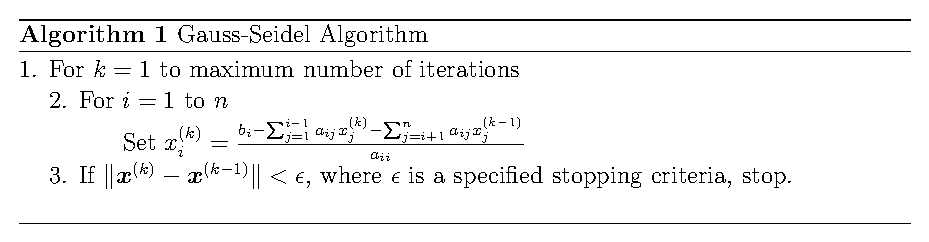
\includegraphics{pictures/algorithm}}%
%{\htmladdimg{pictures/algorithm.png}}
\html{\htmladdimg{pictures/algorithm.pdf}}
\begin{latexonly}
\begin{minipage}{\textwidth}
\hrule height.8pt depth0pt \kern2pt
\noindent\textbf{Thuật toán 1}  Thuật toán Gauss-Seidel \par
\kern2pt\hrule\kern2pt
\begin{tabbing}
1. \=Cho $k=1$ đến các vòng lặp lớn nhất\\
\>2. Cho \=$i=1$ đến $n$\\
\>\>Set 
\begin{math}
x_i^{(k)} = 
\frac{b_i-\sum_{j=1}^{i-1}a_{ij}x_j^{(k)}
         -\sum_{j=i+1}^{n}a_{ij}x_j^{(k-1)}}{a_{ii}}
\end{math}
\\
\>3. Nếu $\|\vec{x}^{(k)}-\vec{x}^{(k-1)}\| < \epsilon$, 
trong đó $\epsilon$ là giới hạn dừng xác định, stop.
\end{tabbing}
\kern2pt\hrule\relax
\end{minipage}
\end{latexonly}
\end{center}

\noindent Dòng sau đây có thể đi sau các hình ảnh và các bảng:
\begin{verbatim}
\listof{algorithm}{Danh sách các thuật toán}
\end{verbatim}
(Bạn có thể \htmladdnormallink{download}{examples/thesis8.tex} \texttt{thesis8.tex} làm một ví dụ.)

%%%%%%%%%%%%%%%%%%%% Generating an Index or Glossary %%%%%%%%%%%%%%%%%%%%

\chapter{Tạo chỉ mục và danh sách các thuật ngữ}

Chúng ta có thể dễ dàng tạo một \Index{Chỉ mục} hoặc \Index{bảng tra cứu thuật ngữ} (danh sách các thuật ngữ) bằng \LaTeX{} và bằng chương trình ứng dụng \Iappname{makeindex}. Một ý tưởng rất hay nếu bạn đưa danh sách các thuật ngữ vào trong một luận án, đặc biệt là nếu có các công thức toán học trong tài liệu của bạn, và  các ký hiệu có thể được giải thích bằng nhiều cách khác nhau.
Ví dụ, $x'$ có thể có nghĩa là $\frac{dx}{dt}$ hoặc nó có thể có nghĩa là một giá trị đã cập nhật của $x$, (hoặc nó có thể là  hoán vị của $x$, nhưng trong trường hợp này $x$ nên được định dạng như một vector). Không có gì khôn ngoan để giả sử rằng người đọc dùng ký hiệu như bạn. Do vậy nên đính kèm một bảng chỉ mục vào trong một luận án, tuy nhiên, \latexbook{} phát biểu rằng bất cứ đề tài không hư cấu nào dài hơn hai mươi trang phải có một bảng chỉ mục.
Nếu bạn chỉ quan tâm đến việc tạo ra một bảng danh sách các thuật ngữ, tôi nghĩ rằng bạn vẫn còn muốn đọc cách làm thế nào để tạo một bảng chỉ mục, danh sách các thuật ngữ và chỉ mục chúng có dạng tương tự sau:


\section{Tạo chỉ mục}

Nếu bạn muốn tạo một chỉ mục, bạn sẽ cần đến lệnh \Com{makeindex} trong phần khai báo (preamble).
Lệnh
\begin{definition}
\Com{index}\{\meta{entry (danh mục)}\}
\end{definition}%
được dùng để lập bảng chú dẫn \meta{entry}  ở một điểm nào đó trong tài liệu. Ví dụ, đoạn mã sau:
\begin{code}
\begin{verbatim}
Các vector riêng\index{vector riêng} được định nghĩa \ldots
\end{verbatim}
\end{code}%
sẽ cho ra output
\begin{result}
Các vector riêng\index{vector riêng} được định nghĩa \ldots
\end{result}%
và đặt danh mục `vector riêng'  trong file \texttt{.idx} file  với số trang liên kết.\\[2.0ex]

\noindent Gói lệnh \sty{makeidx}  cung cấp lệnh \Com{printindex}  mà nó được đặt trong tài liệu nơi mà bạn muốn in ra chỉ mục.
 \noindent Lệnh \Com{makeindex}  sẽ làm cho mỗi lệnh \Com{index} ghi một thông tin xác thực lên file ``\texttt{.idx}''. File này sẽ được xử lý bởi chương trình \appname{makeindex} để tạo ra một file \texttt{.ind} chứa một môi trường \envname{theindex}. Sau đó file này được đọc bởi lệnh \Com{printindex} vào lần biên dịch tài liệu tới. Nếu bạn dùng \appname{TeXnicCenter} bạn sẽ cần chọn ``uses makeindex'' khi bạn tạo một project mới, còn nếu bạn dùng chế độ dòng lệnh bạn cần làm như sau:

\begin{verbatim}
latex filename.tex    
makeindex filename.idx
latex filename.tex
\end{verbatim}
(trong đó \texttt{filename} tên file của tài liệu bạn đang soạn, ví dụ \texttt{thesis})
Nếu bạn cũng đang dùng \BiBTeX, bạn cần tiến hành:
\begin{verbatim}
latex filename.tex
bibtex filename
makeindex filename.idx
latex filename.tex
latex filename.tex
\end{verbatim}

Thật là một ý tưởng hay để tạo các sub-entries (danh mục con) trong bảng chỉ mục, nhằm giúp người đọc dễ dàng tra cứu. Ví dụ, bạn muốn lập danh mục thuật ngữ ``matrix''\index{ma trận} (ma trận), nhưng tài liệu của bạn lại đề cập đến nhiều loại ma trận khác nhau như, ma trận chéo, khối và ma trận cộng tuyến. Trong trường hợp này thì tốt nhất chỉ lập danh mục từ ``matrix'' làm từ tổng quát, và có một danh mục con cho các loại ma trận riêng biệt do vậy danh mục cho từ ``matrix'' được tạo ra sẽ nhìn giống như thế này.  
\begin{description}
\item ma trận, 4, 10, 22--24
\begin{description}
\item chéo, 12
\item khối, 20, 24
\item cộng tuyến, 33
\end{description}
\end{description}
Một danh mục con có thể được tạo ra dùng ký tự \texttt{!}\indextt{"!}. 
Nên danh mục nêu trên được tạo ra dùng các lệnh sau: 
\begin{center}
\begin{tabular}{ll}
Preamble (phần khai báo đầu tài liệu): & \verb|\makeindex|\\ 
Trang 4: & \verb|\index{ma trận}|\\
Trang 10: & \verb|\index{ma trận}|\\
Trang 12: & \verb|\index{ma trận!chéo}|\\
Trang 20: & \verb|\index{ma trận!khối}|\\
Trang 22: & \verb|\index{ma trận}|\\
Trang 23: & \verb|\index{ma trận}|\\
Trang 24: & \verb|\index{ma trận}|\\
Trang 24: & \verb|\index{ma trận!khối}|\\
Trang 33: & \verb|\index{ma trận!cộng tuyến}|\\
Kết thúc văn bản: & \verb|\printindex|
\end{tabular}
\end{center}
 Chú ý rằng cùng các danh mục trên các trang~22,~23 và~24 được chuyển thành  một khoảng~22--24.  Đối với các khoảng lớn hơn bạn có thể chỉ định trang bắt đầu của khoảng bằng cách gắn \verb''|(''  vào chỗ cuối của danh mục trong chỉ mục, gắn vào trang cuối của khoảng trang bằng \verb''|)'' với phần cuối của chỉ mục. 
Ví dụ:
\begin{center}
\begin{tabular}{ll}
Phần khai báo: & \verb|\makeindex|\\ 
Trang 4: & \verb|\index{ma trận}|\\
Trang 10: & \verb|\index{ma trận}|\\
Trang 12: & \verb|\index{ma trận!chéo}|\\
Trang 20: & \verb|\index{ma trận!khối}|\\
Trang 22: & \verb"\index{ma trận|(}"\\
Trang 24: & \verb|\index{ma trận!khối}|\\
Trang 30: & \verb"\index{ma trận|)}"\\
Trang 33: & \verb|\index{ma trận!cộng tuyến}|\\
Kết thúc tài liệu: & \verb|\printindex|
\end{tabular}
\end{center}
sẽ cho ra trong output của index như sau:
\begin{description}
\item ma trận, 4, 10, 22--30
\begin{description}
\item chéo, 12
\item khối, 20, 24
\item cộng tuyến, 33
\end{description}
\end{description}
Một danh sách chỉ mục có thể truy vấn đến một danh mục khác dùng  \verb"|see{"\meta{reference}\verb"}".  Ví dụ,
\begin{verbatim}
\index{Ma trận cộng tuyến|xem{ma trận, cộng tuyến}}
\end{verbatim}
sẽ tạo ra danh mục
\begin{description}
\item ma trận cộng tuyến, \textit{xem} ma trận, cộng tuyến
\end{description}
Định dạng của số trang có thể thay đổi sử dụng \verb"|"\meta{style} trong đó \meta{style} là tên của lệnh định dạng \emph{mà không có} gạch xiên {backslash}. Giả định rằng trong ví dụ trên, định nghĩa của một ma trận được xác định trên trang~10, và do đó bạn có thể muốn số trang xuất hiện ở dạng in đậm để xác định rằng đây là phần tham khảo sơ cấp. Lệnh \verb|\textbf| sẽ in ra chữ in đậm, nên bạn cần gán lệnh \verb|\textbf| vào danh mục trong chỉ mục. Ví dụ, đoạn mã sau:

\begin{center}
\begin{tabular}{ll}
Khai báo: & \verb|\makeindex|\\ 
Trang 4: & \verb|\index{ma trận}|\\
Trang 10: & \verb"\index{ma trận|textbf}"\\
Trang 12: & \verb|\index{ma trận!chéo}|\\
Trang 20: & \verb|\index{ma trận!khối}|\\
Trang 22: & \verb"\index{ma trận|(}"\\
Trang 24: & \verb|\index{ma trận!khối}|\\
Trang 30: & \verb"\index{ma trận|)}"\\
Trang 33: & \verb|\index{ma trận!cộng tuyến}|\\
Kết thúc tài liệu: & \verb|\printindex|
\end{tabular}
\end{center}
sẽ in ra output trong index (chỉ mục) như sau:
\begin{description}
\item ma trận, 4, \textbf{10}, 22--30
\begin{description}
\item chéo, 12
\item khối, 20, 24
\item cộng tuyến, 33
\end{description}
\end{description}

Chương trình \appname{makeindex} sắp xếp chỉ mục theo danh mục đã được xác định, do đó từ ``matrix'' (ma trận) sẽ đứng trước từ ``modulus'', nhưng \verb|$mud$| sẽ được sắp xếp trên các ký tự \verb|$|, \verb|\|, \texttt{m}, \texttt{u} và sau đó là \verb|$|, nên $\mu$ sẽ đứng trước ``matrix''. Điều này có thể không thích hợp, do vậy có thể xác định cách sắp xếp  chỉ mục riêng biệt dùng ký tự \verb|@|\index{''@}:

\begin{verbatim}
\index{mu@$\mu$}
\end{verbatim}
Trong trường hợp này việc sắp xếp được thực hiện trên chuỗi \verb|mu|, nên nó sẽ xuất hiện sau từ ``modulus'', nhưng nó sẽ xuất hiện trong  chỉ mục là $\mu$. Để biết thêm thông tin về cách tạo chỉ mục bạn hãy đọc \latexbook{}, \latexcomp{} hoặc \latexguide.


\subsection{Những vướng mắc thường gặp}
\label{sec:idxproblems}

\begin{itemize}

\item Chỉ mục của tôi không xuất hiện.

\begin{enumerate}
\item Phải chắc chắn rằng bạn dùng lệnh \Com{printindex}  ở vị trí mà bạn muốn chỉ mục được in ra (lệnh này được định nghĩa trong gói \sty{makeidx}).
\item Phải chắc chắn rằng bạn dùng lệnh \Com{makeindex} trong preamble.
\item Bạn phải biên dịch tài liệu bằng \LaTeX\, rồi sau đó chạy \appname{makeindex}, rồi biên dịch lại tài liệu của bạn một lần nữa.
\end{enumerate}

\item Tôi muốn đưa ký tự \verb|@|, \verb"!" hoặc \verb+|+  vào trong chỉ mục nhưng không thấy đâu cả.

Nếu bạn muốn đưa những ký tự này vào chỉ mục bạn cần  bỏ các ký tự này vào dấu trích dẫn kép \verb|''|. Ví dụ:

\begin{verbatim}
\index{"@}
\end{verbatim}
sẽ đưa ký tự \verb|@| vào chỉ mục.

\item Tôi có nhiều danh mục trong một mục. Ví dụ:
\begin{description}
\item matrix, 10, 22-30
\item matrix, 4
\end{description}

Kiểm tra xem  argument bạn dùng cho mỗi lệnh \Com{index} tương ứng phải cùng một argument, chú ý khoảng trắng và lệnh \appname{makeindex} sẽ xử lý các danh mục sau theo những cách khác nhau:

\begin{verbatim}
\index{matrix}
\index{ matrix}
\index{matrix }
\end{verbatim}

\end{itemize}

\section{Tạo một bảng chú giải thuật ngữ}

Có sẵn một số gói lệnh hỗ trợ việc tạo một bảng chú giải thuật ngữ (glossary), đó là các gói \sty{makeglos} (tương tự như các gói lệnh \sty{makeidx}), \sty{glossary}, \sty{glosstex} và \sty{gloss}. Hai gói đầu dùng \LaTeX{} dùng kết hợp với \appname{makeindex}, gói thứ 3   (\sty{glosstex}) dùng \LaTeX{} kết hợp với \appname{makeindex} và \appname{glosstex} trong khi đó gói thứ tư (\sty{gloss}) dùng \LaTeX{} kết hợp với \BiBTeX{}. Tài liệu này chỉ mô tả về \sty{makeglos} và \sty{glossary}, chúng có dạng tương tự như \sty{makeidx}. Nếu bạn quan tâm đến các gói lệnh khác bạn nên đọc các tài liệu đính kèm.
  
\noindent Một bảng chú giải thuật ngữ cũng được tạo ra giống như cách tạo ra một chỉ mục, ngoại trừ bạn dùng lệnh \Com{makeglossary} thay vì dùng \Com{makeindex} và dùng lệnh \Com{glossary} thay cho \Com{index}. Cả hai gói lệnh \sty{makeglos} và \sty{glossary} cung cấp lệnh \Com{printglossary}, tương tự như \Com{printindex}.


\subsection{Gói lệnh \latexhtml{\texorpdfstring{\sty{makeglos}}{makeglos}}{\sty{makeglos}}}

Xem xét ví dụ sau:
\begin{center}
\begin{tabular}{ll}
Khai báo : & \verb|\makeglossary|\\
Trang 2 : & \verb"\glossary{tập hợp: một bộ sưu tập các đối tượng}"\\
Trang 3 : & \verb"\glossary{phần tử: số đối tượng trong một tập hợp}"\\
Trang 4 : & \verb"\glossary{tập hợp hỗn tạp: chứa mọi thứ}"
\end{tabular}
\end{center}
\noindent Biên dịch tài liệu này sẽ tạo ra một file với tên mở rộng \texttt{.glo} chứa thông tin chi tiết về bảng chú giải thuật ngữ. Bạn có thể dùng chương trình \appname{makeindex} để xử lý những danh mục trong bảng này, nhưng bạn cần điều chỉnh một chút.


\begin{enumerate}
\item Bạn cần tạo một \appname{makeindex}
style file (file phong cách)  mới mà nó thông báo cho \appname{makeindex} tìm kiếm \Com{danh mục thuật ngữ} thay vì \Com{danh mục trong chỉ mục}, và tạo môi trường \envname{theglossary} thay cho môi trường \envname{theindex}.
Hãy gọi \appname{makeindex} style file mới này là \verb|thesisglo.ist|. Đầu tiên chúng ta cần đặt từ khóa \verb|"\\glossaryentry"|:

\begin{verbatim}
từ kóa "\\glossaryentry"
\end{verbatim}
bây giờ chúng ta cần thay đổi khai báo sang \verb|"\\begin{theglossary}\n"| và phần khai báo phụ trợ \latex{\ifscreen\else\linebreak\fi}
\verb|"\n\n\\end{theglossary}\n"|:
\begin{verbatim}
khai báo "\\begin{theglossary}\n"
khai báo phụ trợ "\n\n\\end{theglossary}\n"
\end{verbatim}
Bây giờ chúng ta cần thông báo cho \appname{makeindex} dùng phong cách này sử dụng chọn lựa \verb|-s|, và bạn cũng cần định rõ file output, nó nên có dạng mở rộng là \verb|.gls|, sử dụng chọn lựa \verb|-s|:

\begin{verbatim}
makeindex -o thesis.gls -s thesisglo.ist thesis.glo
\end{verbatim}
(Giả sử rằng tài liệu chính có chứa file\verb|thesis.tex|  và bạn đã chạy \LaTeX{} trước khi gọi  chương trình \appname{makeindex}.) 
Chú ý rằng bạn đang dùng \verb|thesis.glo| (đã được tạo ra bởi  các lệnh \Com{glossary}) mà không phải là file \verb"thesis.idx" (được tạo ra bởi các lệnh \Com{index})


\item Theo mặc định, \appname{makeindex}  sẽ dùng file với phần mở rộng là \verb|.ilg| như log file, có thể bạn muốn đổi file này để tránh xung đột với index log file. Ví dụ, bạn muốn gọi log file của bảng chú giải thuật ngữ \verb|thesis.glg|:

\begin{verbatim}
makeindex -t thesis.glg -o thesis.gls -s thesisglo.ist thesis.glo
\end{verbatim}

\end{enumerate}

Đây là một ví dụ dùng gói \sty{makeglos}:\\[10pt]
File \texttt{sample.tex}:

\begin{verbatim}
\documentclass[a4paper]{report}
\usepackage{makeglos}
\makeglossary
\begin{document}
\printglossary

\chapter{Giới thiệu}
Một tập hợp\glossary{tập hợp: Bộ sưu tập các đối tượng} 
thường được biểu thị trong một  font thư pháp, 
ví dụ $\mathcal{S}$. 
Phần tử của tập hợp\glossary{phần tử của tập hợp: 
Số các đối tượng trong tập hợp} của $\mathcal{S}$ 
được kí hiệu là $|\mathcal{S}|$. 
Tập hợp hỗn tạp\glossary{tập hợp hỗn tạp: 
Chứa mọi thứ} thì thường được kí hiệu là $\mathcal{U}$
\end{document}
\end{verbatim}

File của \appname{makeindex}  là style file, \texttt{sample.ist}, sẽ giống như thế này:
\begin{verbatim}
từ khóa "\\glossaryentry"
khai báo "\\begin{theglossary}\n"
khai báo bổ trợ "\\end{theglossary}\n"
\end{verbatim}

Sau đó bạn cần thực hiện
\begin{verbatim}
latex sample.tex % biên dịch file sample.tex
makeindex -t sample.glg -o sample.gls -s sample.ist sample.glo
% tạo chỉ mục, bảng tra cứu thuật ngữ theo các lựa chọn.
latex sample.tex % biên dịch lại file sample.tex
\end{verbatim}

\noindent Tiêu đề của bảng tra cứu thuật ngữ (tên mặc định là: Glossary)  có thể thay đổi bằng cách định nghĩa lại  lệnh \Com{glossaryname}.  Nếu bạn muốn bất cứ đoạn văn bản nào xuất hiện ở đầu bảng tra cứu thuật ngữ bạn chỉ cần định nghĩa lại lệnh \Com{glossaryintro}.  Định dạng của argument cho lệnh \Com{glossary} command thì tương tự như với \Com{index}, do đó bạn có thể dùng \verb|@| để chỉ cách sắp xếp danh mục, dùng \verb"|" để chỉ định làm cách nào để định dạng  số trang liên đới và \verb|!| dùng để xác định các danh mục con (mặc dù điều này không thích hợp cho một bảng tra cứu thuật ngữ). Nếu bạn gặp rắc rối, hãy tham khảo mục~\ref{sec:idxproblems} để tìm biện pháp tháo gỡ 
\latex{\ifscreen \else\ trên trang~\pageref{sec:idxproblems}\fi}.

Bạn cũng có thể download file sau: 
\htmladdnormallink{thesis9.tex}{examples/thesis9.tex} và
\htmladdnormallink{thesisglo.ist}{examples/thesisglo.ist} sẽ minh họa cho ví dụ này.

%------------ glossary.sty ----------------

\subsection{Gói lệnh \latexhtml{\texorpdfstring{\sty{glossary}}{glossary}}{\sty{glossary}}}

Gói lệnh \sty{glossary} cũng định nghĩa lệnh \Com{printglossary}, nhưng nó định nghĩa lại lệnh \Com{glossary}  đó bạn có thể tách tên của danh mục và  mô tả tương ứng của nó, dùng một tập hợp của \meta{từ khóa}= cặp \meta{giá trị}.
\noindent Những key sau đây luôn sẵn có:
\begin{center}
\begin{tabular}{ll}
tên & Tên của danh mục\\
mô tả & Một mô tả của danh mục\\
sắp xếp & Làm sao để sắp xếp danh mục. (Danh mục thường được đặt tên theo mặc định)\\
định dạng & Cách định dạng số trang
\end{tabular}
\end{center}
Ví dụ ở phần trên có thể thay đổi thành:
\begin{htmlonly}
\begin{center}
\begin{tabular}{ll}
Khai báo : & \verb|\makeglossary|\\
Trang 2 : & \verb"\glossary{tên = tập hợp,mô tả = một bộ sưu tập các đối tượng}"\\
Trang 3 : & \verb"\glossary{tên=phần tử của tập hợp,mô tả = số đối tượng trong một tập hợp}"\\
Trang 4 : & \verb"\glossary{tên = tập hợp hỗn tạp, mô tả =tập hợp chứa mọi thứ}"
\end{tabular}
\end{center}
\end{htmlonly}

\begin{latexonly}
\begin{center}
\begin{tabular}{ll}
Khai báo : & \verb|\makeglossary|\\
Trang 2 : & \verb"\glossary{tên = tập hợp,mô tả = một bộ"\\
         & \verb"          sưu tập các đối tượng}"\\
Trang 3 : & \verb"\glossary{tên = phần tử của tập hợp, mô tả = số"\\
         & \verb"          đối tượng trong một tập hợp}"\\
Trang 4 : & \verb"\glossary{tên = tập hợp hỗn tạp, mô tả ="\\
         & \verb"          tập hợp chứa mọi thứ}"
\end{tabular}
\end{center}
\end{latexonly}

\noindent Gói lệnh \sty{glossary} tạo style file \appname{makeindex} \texttt{.ist} style file để tùy biến cho tài liệu của bạn, nên bạn không cần lo lắng để tạo nó nữa. Theo mặc định tên của file \texttt{.ist} sẽ có cùng tên gốc với tên tài liệu của bạn, do đó nếu tài liệu của bạn có tên là \texttt{sample.tex} thì file này sẽ có tên là \texttt{sample.ist} tên này sẽ được tạo ra khi bạn biên dịch file gốc \texttt{sample.tex}. Như trên bạn cần làm:

\begin{verbatim}
latex sample.tex % biên dịch file sample.tex
makeindex -t sample.glg -o sample.gls -s sample.ist sample.glo
% tạo chỉ mục, bảng tra cứu thuật ngữ theo các lựa chọn.
latex sample.tex % biên dịch lại file sample.tex
\end{verbatim}
Bạn có thể dùng Perl script \appname{makeglos}  được cung cấp trong   version 2.0 của gói lệnh \sty{glossary}:

\begin{verbatim}
latex sample.tex
makeglos sample.glo
latex sample.tex
\end{verbatim}

Phong cách của bảng tra cứu thuật ngữ có thể tùy biến.  Như trên tiêu đề của bảng tra cứu các thuật ngữ (tên mặc định là Glossary) có thể thay đồi bằng cách định nghĩa lại lệnh \Com{glossaryname}. Phong cách của bảng tra cứu thuật ngữ có thể thay đổi dùng các lựa chọn của gói lệnh mà các lựa chọn này có dạng \meta{từ khóa}=\meta{giá trị}:

\begin{description}
\item[style] Phong cách của môi trường \envname{theglossary}. Các giá trị:
\begin{description}
\item[list] dùng môi trường mô tả trong bảng tra cứu thuật ngữ
\item[super] dùng môi trường supertabular (bạn là người sử dụng \TeX{} chắc bạn biết tabular nghĩa là gì rồi) trong bảng tra cứu thuật ngữ
\item[long] dùng môi trường bảng dài trong bảng tra cứu thuật ngữ (mặc định)
\end{description}

\item[header] header của bảng tra cứu thuật ngữ. Các giá trị:
\begin{description}
\item[none] bảng tra cứu thuật ngữ không có tiêu đề trang (Mặc định)
\item[plain] bảng tra cứu thuật ngữ có tiêu đề trang
\end{description}

\item[border] Đường viền của Bảng tra cứu thuật ngữ. Các giá trị:
\begin{description}
\item[none] Bảng tra cứu thuật ngữ  không có đường viền (Mặc định)
\item[plain] Đường viền xung quanh của Bảng tra cứu thuật ngữ
\end{description}

\item[cols] Số cột. Các giá trị:
\begin{description}
\item[2] Tên của danh mục và chú giải nằm ở hai cột riêng biệt,  với số trang liên đới nằm cùng cột với chú giải  (Mặc định). 
\item[3] Tên danh mục, chú giải và các trang liên đới nằm trong ba cột riêng biệt.
\end{description}

\item[number] Số trang liên đới tương ứng với mỗi  giá trị của danh mục\footnote{lựa chọn này chỉ có trong version 1.1 và các version sau này}.
Các giá trị :
\begin{description}
\item[page] Mỗi danh mục ở một trang tương ứng nơi mà danh mục được đặt. (Mặc định)
\item[section] Mỗi danh mục được đánh số một mục tương ứng nơi mà danh mục được định nghĩa.
\item[none] Các con số tương ứng được lược bớt.
\end{description}

\item[toc] Biến boolean\footnote{lựa chọn này sẵn có trong version 2.0 và các version sau này}
\begin{description}
\item[true] In Bảng tra cứu thuật ngữ vào mục lục
\item[false] Không in Bảng tra cứu thuật ngữ vào mục lục (mặc định)
\end{description}
Chú ý rằng nếu bạn định rõ lựa chọn này bạn cần  biên dịch lại tài liệu thêm hai lần nữa sau khi tạo Bảng tra cứu thuật ngữ.


\item[hyper] Biến boolean\footnote{lựa chọn này sẵn có trong version 2.0511 và các phiên bản sau này}
\begin{description}
\item[true] Tạo các số liên đới với một liên kết siêu văn bản
\item[false] Không tạo các số liên đới với một liên kết siêu văn bản
\end{description}
Nếu gói lệnh \sty{hyperref} được tải trước khi tải gói \sty{glossary} thì \texttt{hyper=true} được đặt, nếu không nó sẽ được đặt mặc định \texttt{hyper=false}.
\end{description}
Các lựa chọn \texttt{border}, \texttt{header} and \texttt{cols} không nên dùng trong việc liên kết với  \texttt{style=list}, chúng chỉ có nghĩa với lựa chọn kiểu bảng. 
Ví dụ:
\begin{verbatim}
\usepackage[style=long,cols=3,border=plain]{glossary}
\end{verbatim}

Nếu bạn muốn chèn thêm thông tin ở đầu hay cuối bảng tra cứu thuật ngữ bạn có thể định nghĩa lại các lệnh \Com{glossarypreamble} và \Com{glossarypostamble}. Bạn cũng có thể định nghĩa thêm các đối tượng phong cách cho bảng tra cứu thuật ngữ, nên bạn sẽ có thêm lựa chọn cho cách trình bày bảng tra cứu thuật ngữ trong tài liệu của bạn. Ví dụ, một bảng tra cứu của một số thuật ngữ và một chỉ mục của các hàm toán hoặc  của các ký hiệu.
Bạn có thể download version mới nhất của gói lệnh \sty{glossary} tại 
\url{http://theoval.cmp.uea.ac.uk/~nlct/latex/packages/index.html#glossary}.

Download \download{thesis10} \texttt{thesis10.tex} làm ví dụ.

%%%%%%%%%%%%%%%%%%%% Too Many Unprocessed Floats %%%%%%%%%%%%%%%%%%%%%%%%

\chapter{Nhiều float không được xử lý }
Một vấn đề chung mà các nghiên cứu sinh thường gặp khi viết luận án là có báo lỗi ``Nhiều Float Không Được Xử Lý''. Lỗi này phát sinh do có quá nhiều hình ảnh và bảng trong ``Chương kết quả nghiên cứu'' và không có nhiều dòng chữ được nhập vào xung quanh chúng. Nếu điều này xảy ra thì có một số biện pháp mà bạn có thể thử: 


\begin{enumerate}
\item Kiểm tra xem bạn chưa giới hạn chính xác vị trí mà  bạn muốn đặt float.  Nếu bạn xác định chính xác vị trí thì hãy cho \LaTeX{} nhiều lựa chọn nếu có thể.
Ví dụ:
\begin{verbatim}
\begin{figure}[htbp]
\end{verbatim}
Điều này có thể xác định rằng bạn có thể chèn hình ảnh vào tại điểm bạn đang làm việc ``h=here'', hay ở trên đầu trang ``t=top'', ở phía dưới của trang ``b=bottom'', hoặc trên một trang chỉ chứa hình ảnh thuần túy ``p=page''

\item Hãy cố gắng tăng số lượng văn bản trong một chương. Nhớ rằng bạn không nên  cho hiển thị tất cả các hình ảnh và bảng biểu trong chương ``Kết quả khảo sát'' mà không tham vấn với người hướng dẫn.

\item Nếu tất cả các biện pháp mà bạn áp dụng không thay đổi được tình thế, thì cố gắng dùng lệnh \Com{clearpage}.  Lệnh này buộc tất cả các float chưa xử lý được thì sẽ được xử lý lại tức thời, và bắt đầu một trang mới. Nhưng có thể làm trang bị ngắt đột ngột, để tránh điều này bạn có thể dùng gói lệnh \sty{afterpage} của David~Carlisle và sử dụng lệnh:  
\begin{verbatim}
\afterpage{\clearpage}
\end{verbatim}
\end{enumerate}

Nếu còn những vướng mắc chưa giải quyết được, tham khảo phần FAQ trên \TeXarchive.

%%%%%%%%%%%%%%%%%%%%%%%%%%% Tài liệu tham %khảo%%%%%%%%%%%%%%%%%%%%%%%%%%%%%%%%

\begin{thebibliography}{1}
\latex{\addcontentsline{toc}{chapter}{Tài liệu tham khảo}}
\label{ch:bib}

\bibitem{goossens94} ``The \LaTeX\ Companion'', Michel Goossens, Frank Mittelbach and
Alexander Samarin, Addison-Wesley (1994).

\bibitem{kopka95} ``A Guide to \latexhtml{\LaTeX 2$\varepsilon$}{\LaTeX2e}: document preparation for beginners
and advanced users'', Helmut Kopka and Patrick W. Daly, Addison-Wesley (1995).

\bibitem{lamport94} ``\LaTeX\ : a document preparation system'', Leslie~Lamport, 2nd ed.\ Addison-Wesley (1994).

\bibitem{texarchive} The \TeX\ Archive. \url{http://www.tex.ac.uk/}\index{TeX Archive@\TeX\ Archive}

\begin{latexonly}
\bibitem{novices} ``LaTeX for Complete Novices'', Nicola Talbot. 
\url{http://theoval.cmp.uea.ac.uk/~nlct/latex/novices/} (2004).
\end{latexonly}

\end{thebibliography}
\renewcommand{\indexname}{Chỉ mục}
\printindex

\end{document}

